\documentclass[12pt,a4paper,bibliography=totocnumbered,listof=totoc]{scrartcl}
\usepackage[ngerman]{babel}
\usepackage[T1]{fontenc}% wichtig für Trennung von Wörtern mit Umlauten
\usepackage{microtype}% verbesserter Randausgleich
\usepackage[utf8]{inputenc}
\usepackage{amsmath}
\usepackage{amsfonts}
\usepackage{amssymb}
\usepackage{graphicx}
\usepackage{fancyhdr}
\usepackage{tabularx}
\usepackage{geometry}
\usepackage{setspace}
\usepackage[right]{eurosym}
\usepackage[printonlyused]{acronym}
\usepackage{subfig}
\usepackage{floatflt}
\usepackage[usenames,dvipsnames]{color}
\usepackage{colortbl}
\usepackage{paralist}
\usepackage{array}
\usepackage{titlesec}
\usepackage{parskip}
\usepackage[right]{eurosym}
\usepackage{picins}
\usepackage[subfigure,titles]{tocloft}
\usepackage[pdfpagelabels=true]{hyperref}
\usepackage{natbib}
\bibliographystyle{dinat}

\usepackage{listings}
\lstset{basicstyle=\footnotesize, captionpos=b, breaklines=true, showstringspaces=false, tabsize=2, frame=lines, numbers=left, numberstyle=\tiny, xleftmargin=2em, framexleftmargin=2em}
\makeatletter
\def\l@lstlisting#1#2{\@dottedtocline{1}{0em}{1em}{\hspace{1,5em} Lst. #1}{#2}}
\makeatother

\geometry{a4paper, top=27mm, left=30mm, right=30mm, bottom=35mm, headsep=10mm, footskip=12mm}

\hypersetup{unicode=false, pdftoolbar=true, pdfmenubar=true, pdffitwindow=false, pdfstartview={FitH},
	pdftitle={Abschlussarbeit},
	pdfauthor={Philipp Anders},
	pdfsubject={Bachelorarbeit},
	pdfcreator={\LaTeX\ with package \flqq hyperref\frqq},
	pdfproducer={pdfTeX \the\pdftexversion.\pdftexrevision},
	pdfkeywords={Bachelorarebti},
	pdfnewwindow=true,
	colorlinks=true,linkcolor=black,citecolor=black,filecolor=magenta,urlcolor=black}
\pdfinfo{/CreationDate (D:20110620133321)}

\begin{document}

\titlespacing{\section}{0pt}{12pt plus 4pt minus 2pt}{-6pt plus 2pt minus 2pt}

% Kopf- und Fusszeile
\renewcommand{\sectionmark}[1]{\markright{#1}}
\renewcommand{\leftmark}{\rightmark}
\pagestyle{fancy}
\lhead{}
\chead{}
\rhead{\thesection\space\contentsname}
\lfoot{}
\cfoot{}
\rfoot{\thepage}
\renewcommand{\headrulewidth}{0.4pt}
% \renewcommand{\footrulewidth}{0.4pt}

% Vorspann
\renewcommand{\thechapter}{\Roman{chapter}}
\pagenumbering{Roman}
\raggedbottom

% ----------------------------------------------------------------------------------------------------------
% Titelseite
% ----------------------------------------------------------------------------------------------------------
\thispagestyle{empty}
\begin{center}
	\vspace*{1cm}
	\textbf{Hochschule für Technik, Wirtschaft und Kultur Leipzig}\\
	\vspace*{0.3cm}
	Fakultät Informatik, Mathematik und Naturwissenschaften\\
	Bachelorstudiengang Medieninformatik\\
	\vspace*{1cm}
	Bachelorarbeit\\
	zur Erlangung des akademischen Grades\\
	\vspace*{0.3cm}
	\textbf{Bachelor of Science (B.Sc.)}\\
	\Huge
	\vspace*{1cm}
	\textbf{Integration des Tacton Produktkonfigurators in ein Open Source Shopsystem}\\
	
	\vfill
	\normalsize
	\newcolumntype{x}[1]{>{\raggedleft\arraybackslash\hspace{0pt}}p{#1}}
	\begin{tabular}{x{3cm}p{10cm}}
		\rule{0mm}{5ex}\textbf{eingereicht von:} & Philipp Anders\newline Matrikelnummer: 58359 \\ 
		\rule{0mm}{5ex}\textbf{Betreuer:} & Prof. Dr. Michael Frank (HTWK Leipzig)\newline Dipl.-Wirt.-Inf. (FH) Dirk Noack (Lino GmbH)\\ 
		\rule{0mm}{5ex}\textbf{Abgabedatum:} & 28.09.2015 \\ 
	\end{tabular} 
\end{center}
\pagebreak

% ----------------------------------------------------------------------------------------------------------
% Abstract
% ----------------------------------------------------------------------------------------------------------
\setcounter{page}{1}
\onehalfspacing
\titlespacing{\section}{0pt}{12pt plus 4pt minus 2pt}{2pt plus 2pt minus 2pt}
\section*{Kurzfassung}
Das ganze auf Deutsch.

\vspace{-1,2em}
\titlespacing{\section}{0pt}{12pt plus 4pt minus 2pt}{-6pt plus 2pt minus 2pt}
\section*{Abstract}
Das ganze auf Englisch.
\pagebreak

% ----------------------------------------------------------------------------------------------------------
% Verzeichnisse
% ----------------------------------------------------------------------------------------------------------
% TODO Typ vor Nummer
\renewcommand{\cfttabpresnum}{Tab. }
\renewcommand{\cftfigpresnum}{Abb. }
\settowidth{\cfttabnumwidth}{Abb. 10\quad}
\settowidth{\cftfignumwidth}{Abb. 10\quad}

\rhead{Inhaltsverzeichnis}
\setcounter{secnumdepth}{3} 
\setcounter{tocdepth}{3}
\tableofcontents
\pagebreak
\rhead{Verzeichnisse}
\listoffigures
\pagebreak
\listoftables
\pagebreak
\renewcommand{\lstlistlistingname}{Listing-Verzeichnis}
\lstlistoflistings
\pagebreak

% ----------------------------------------------------------------------------------------------------------
% Abkürzungen
% ----------------------------------------------------------------------------------------------------------
\chapter*{Abkürzungsverzeichnis}
\addcontentsline{toc}{chapter}{Abkürzungsverzeichnis} 
\begin{acronym}[WSDL] % längste Abkürzung steht in eckigen Klammern
	\setlength{\itemsep}{-\parsep} % geringerer Zeilenabstand
	\acro{AJAX}{asynchronous JavaScript and XML}
	\acro{API}{Application Programming Interface}
	\acro{ATO}{Assemble-to-Order}
	\acro{B2B}{Business-to-Business}
	\acro{B2C}{Business-to-Customer}
	\acro{CORS}{Cross-Origin Resource Sharing}
	\acro{CSP}{Constraint Satisfaction Problem}
	\acro{etc.}{et cetera}
	\acro{ETO}{Engineer-to-Order}
	\acro{i.d.R.}{in der Regel}
	\acro{JSON}{JavaScript Object Notation}
	\acro{MC}{Mass Customization}
	\acro{MTO}{Make-to-Order}
	\acro{MVC}{Model View Controller}
	\acro{ORM}{objektrelationale Abbildung}
	\acro{PTO}{Pick-to-Order}
	\acro{RPC}{Remote Procedure Call}
	\acro{SOP}{Same-Origin-Policy}
	\acro{UML}{Unified Modeling Language}
	\acro{URI}{Uniform Resource Identifier}
	\acro{vgl.}{vergleiche}
	\acro{WSDL}{Web Service Description Language}
\end{acronym}
\newpage

% ----------------------------------------------------------------------------------------------------------
% Inhalt
% ----------------------------------------------------------------------------------------------------------
% Abstände Überschrift
\titlespacing{\section}{0pt}{12pt plus 4pt minus 2pt}{0pt plus 2pt minus 2pt}
\titlespacing{\subsection}{0pt}{12pt plus 4pt minus 2pt}{-1pt plus 2pt minus 2pt}
\titlespacing{\subsubsection}{0pt}{12pt plus 4pt minus 2pt}{-1pt plus 2pt minus 2pt}

% Kopfzeile
\renewcommand{\sectionmark}[1]{\markright{#1}}
\renewcommand{\subsectionmark}[1]{}
\renewcommand{\subsubsectionmark}[1]{}
\lhead{Kapitel \thesection}
\rhead{\rightmark}

\onehalfspacing
\renewcommand{\thesection}{\arabic{section}}
\renewcommand{\theHsection}{\arabic{section}}
\setcounter{section}{0}
\pagenumbering{arabic}
\setcounter{page}{1}


\section{Einleitung}

\subsection{Ziel der Arbeit}

\subsection{Aufbau der Arbeit}

\pagebreak

\section{Grundlagen}

\subsection{Konfiguration}
Im Folgenden Abschnitt wird geklärt: was ist ein Konfigurator und wofür brauchen wir ihn? Aus Gründen der Nachvollziehbarkeit werden diese Fragen allerdings in umgedrehter Reihenfolge bearbeitet.
Dazu wird zunächst eine marktwirtschaftliche Situation erläutert, welche die Notwendigkeit hybrider Wettbewerbsstrategien begründet. Diese wiederum stellen zu ihrer Umsetzbarkeit Bedingungen an Produktionskonzepte, welche daraufhin vorgestellt werden. Abschließend wird geklärt, welchen Beitrag die Produktkonfiguration dabei leistet und dessen Funktionsweise erläutert.

\subsubsection{Anwendungsrahmen}
 \label{subssubsection:Ausgangssituation}
Neue Wettbewerbsbedingungen und gesteigerte Kundenansprüche haben den Druck auf Industrieunternehmen zur Produktion individualisierter Produkte erhöht \citep{piller98}. Dies erfordert eine stärkere Leistungsdifferenzierung\citep{lutz11}. Die Differenzierung ist ein der von \citeauthor{porter02} beschriebenen \glqq generischen Wettbewerbsstrategien\grqq{}. Weitere sind die Kostenführerschafts- und Fokussierungsstrategie. Die Kostenführerschaft bezieht sich klassischerweise auf Anbieter von Massenproduktion. Durch die Unterbietung der Konkurrenzpreise wird der Marktanteil erhöht. Dem Gegenüber entspricht die Leistungsdifferenzierung dem Verkauf von Produkten mit höherem individuellen Kundennutzen zu höheren Preisen.

\vspace{1em}
\begin{minipage}{\linewidth}
	\centering
	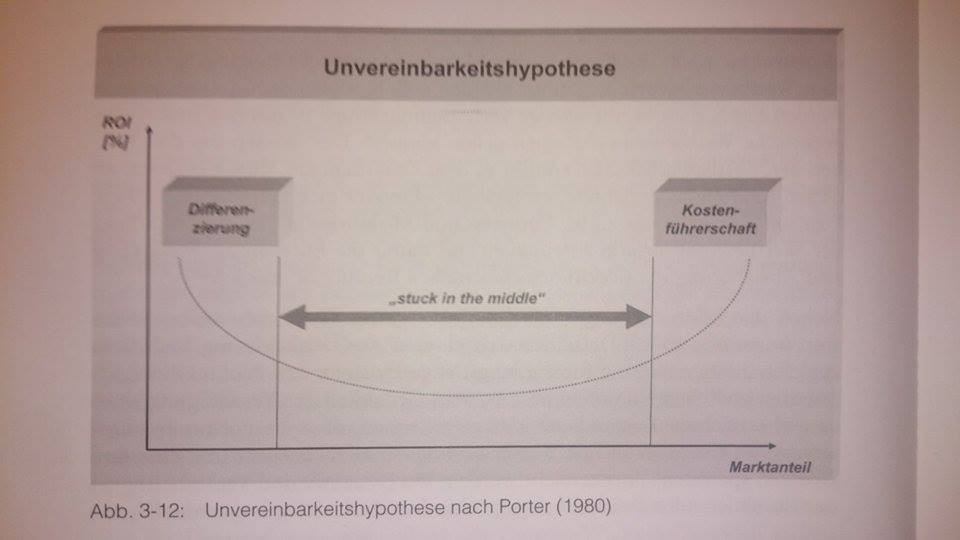
\includegraphics[width=0.7\linewidth]{Abbildungen/unvereinbarkeitshypothese.jpg}
	\captionof{figure}[Unvereinbarkeitshypothese]{Unvereinbarkeitshypothese nach \cite{porter80}, zitiert von \cite{schuh05}}
	\label{fig:unvereinbarkeitshypothese}
\end{minipage}
\vspace{1em}

In diesem Zusammenhang formulierte \citeauthor{porter80} die Unvereinbarkeitshypothese. So sollen Kostenführerschaft und Leistungsdifferenzierung nicht gleichzeitig erreichbar sein. Eine uneindeutige Positionierung führe zu einem \glqq stuck in the middle\grqq{} und damit zur Unwirtschaftlichkeit, wie Abbildung \ref{fig:unvereinbarkeitshypothese} darstellt.

Die Beobachtung der Unternehmensrealität zeichnet jedoch ein anderes Bild. Neue Organisatzionsprinzipien, Informationsverarbeitungspotentiale und Produktstrukturierungsansätze ermöglichen einen Kompromiss aus Preis- und Leistungsführerschaft \citep{schuh05}. Das Ergebnis wird als hybride Wettbewerbsstrategien bezeichnet. Eine dieser Strategien ist die sogenannte \ac{MC}.

\ac{MC} ist die \glqq Produktion von Gütern und Leistungen für einen (relativ) großen Absatzmarkt, welche die unterschiedlichen Bedürfnisse jedes einzelnen Nachfragers dieser Produkte treffen, zu Kosten, die ungefähr denen einer massenhaften Fertigung vergleichbarer Standardgüter entsprechen\grqq{} \citep{piller98}. Mit anderen Worten: Preisvorteil (i.d.R. durch Massenfertigung) wird mit Individualisierung (i.d.R. durch Variantenvielfalt) verbunden.

\subsubsection{Produktklassifizierung}
 \label{subssubsection:Produktklassifizierung}

\ac{MC} setzt zu deren Umsetzbarkeit gewisse Bedingungen an die Produktionsweisen der abgesetzten Güter. Im Folgenden wird eine Klassifizierung von Produkten in Bezug auf deren Herstellung vorgestellt, was von \citet{schuh06} als Produktionskonzepte bezeichnet wird. Abgestimmt auf diese Produktionskonzepte lässt sich daraufhin der jeweilige Nutzen einer Produktkonfiguration ableiten.

Folgende Produktionskonzepte werden unterschieden (nach \citealt{schuh06}, zitiert von \citealt{lutz11}):
\begin{compactitem}
	\item \textbf{\ac{PTO}:} Herstellung ohne Kundenauftrag. Lagerhaltung ganzer Produkte. Keine Abhängigkeit dieser Produkte untereinander. Keine Berücksichtigung von Kundenanforderungen.
	\item \textbf{\ac{ATO}:} Herstellung ohne Kundeauftrag. Lagerhaltung von Baugruppen/-teilen. Teile mit Abhängigkeiten untereinander. Berücksichtigung von Kundenanforderungen.
	\item \textbf{\ac{MTO}:} Herstellung teilweise erst nach Kundenenauftrag. Lagerhaltung von standardisierten Baugruppen/-teilen sowie Produktion von vorgedachten Komponenten nach Kundenanforderung. Abhängigkeiten zwischen Teilen. Keine unendliche Anzahl von Varianten.
	\item \textbf{\ac{ETO}:} Herstellung erst nach Kundenauftrag. Wenig Lagerhaltung von Baugruppen/-teilen. Entwicklung und Fertigung von Teilen nach Kundenspezifikation. Unendliche Variantenanzahl möglich.
\end{compactitem}

Die Produktionskonzepte unterscheiden sich hauptsächlich nach dem Kriterium, wann die Produktion der Baugruppen/-teile beginnt - vor oder nach Auftragsspezifikation. Eine Produktion vor Auftragseingang, also ohne Kundenspezifikation, erlaubt Lagerhaltung. Die Einflussnahme des Kunden auf das Endprodukt - abgesehen von der Kaufentscheidung - beginnt bei \ac{ATO}. \citeauthor{lutz11} kommt zu dem Schluss, dass \ac{MTO} am ehesten der Definition individualisierter Güter im Rahmen der \ac{MC} entspricht. Während sie einen Grundanteil standardisierter Komponenten besitzen, sind sie doch im ausreichenden Maße durch den Kunden anpassbar.

\textbf{Zwischenfazit}\\
In Abschnitt \ref{subssubsection:Produktklassifizierung} wurde dargestellt, wie bestimmte Produktionskonzepte die Herstellung individualisierter Produktvarianten bei gleichzeitiger Lagerfertigung ermöglichen. Produkte werden mit dem Ziel gestaltet, so individuell und auftragsunabhängig wie möglich zu sein. Damit wurde eine der Schlüsselfaktoren für die Ermöglichung der hybriden Wettbewerbsstrategie \ac{MC} erläutert. Diese verbindet die Vorteile effizienter Massenproduktion mit denen
der kundenspezifischen Einzelfertigung\citep{piller98}.

\subsubsection{Produktkonfiguration}
 \label{subssubsection:Produktkonfiguration}
 
Aus der im vorangegangenen Kapitel vorgestellten \ac{MC} resultiert mehr Produktvariabilität und damit mehr Produktkomplexität. Die Produktkonfiguration (Konfiguration) ist ein Werkzeug zur Beherrschung dieser Komplexität. Sie unterstützt das Finden einer Produktvariante, die auf Kundenanforderungen angepasst und gleichzeitig machbar ist \citep{lutz11}. Diese wird von einem Produktkonfigurationssystem (Konfigurator) durchgeführt. Es folgt nun eine Definition der in diesem Zusammenhang wichtigen Begriffe.

\textbf{Begriffsüberblick}\\
\textbf{Konfiguration} ist eine spezielle Designaktivität, bei der der zu konfigurierende Gegenstand aus Instanzen einer festen Menge wohldefinierter Komponententypen zusammengesetzt wird, welche entsprechend einer Menge von Konfigurationsregeln kombiniert werden können \citep{sabin98}.

Die Einordnung als Designaktivität erlaubt außerdem die Beschreibung der Konfiguration als ein Designtyp. Es werden das \glqq Routine Design\grqq{}, \glqq Innovative Design\grqq{} und \glqq Creative Design\grqq{} unterschieden. Die Konfiguration entspricht dem \glqq Routine Design\grqq{}. Dabei handelt es sich um ein Problem, bei der die Spezifikation der Objekte, deren Eigenschaften sowie kompositionelle Struktur gegeben sind und die Lösung auf Basis einer bekannten Strategie gefunden wird \citep{brown89}. Damit ist \glqq Routine Design\grqq{} die simpelste der drei Formen. Die anderen Designtypen enthalten hingegen Objekte und Objektbeziehungen, die erst während des Designprozesses entwickelt werden., 

Die Schlüsselbegriffe der Definition von \citeauthor{sabin98} sind Komponententypen und Konfigurationsregeln. \textbf{Komponententypen} sind Kombinationselemente, welche durch Attribute charakterisiert werden und eine Menge alternativer (konkreter) Komponenten repräsentieren. Übertragen auf die objektorientierte Programmierung verhalten sich Komponententypen zu Komponenten wie Klassen zu Instanzen. Komponententypen stehen zueinander in Beziehung. Diese kann entweder eine \glqq Teil-Ganzes\grqq{}-Beziehung oder Generalisierung sein \citep{felferning14}. 

\textbf{Konfigurationsregeln} (Constraints) im engeren Sinne sind Kombinationsrestriktionen \citep{felferning14}. Weitere Arten werden später vorgestellt.

Zur besseren Nachvollziehbarkeit den weiteren Terminologie ist eine Definition des Variantenbegriffs angebracht. DIN 199 beschreibt Varianten als \glqq Gegenstände ähnlicher Form und/oder Funktion mit einem in der Regel hohen Anteil identischer Gruppen oder Teile\grqq{}. Damit ist also eine Gegenstandsmenge gemeint. Ein Element dieser Menge ist demzufolge eine konkrete Variantenausprägung. Eine Variantenausprägung unterscheidet sich von einer anderen durch mindestens eine Beziehung oder ein Element \citep{lutz11}.

Die Einheit aus Komponententypen sowie das Wissen um deren Kombinierbarkeit in Form von Constraints wird als \textbf{Konfigurationsmodell} bezeichnet. Es bildet die Menge der validen Lösungen und definiert so implizit alle Variantenausprägungen eines Produktes. Dadurch muss nicht jede Variantenausprägung explizit definiert und abgespeichert werden (z.B. in einer Datenbank). Die Anzahl möglicher Kombinationen kann in die Millionen gehen, was die Suche nach einer bestimmten sehr zeitaufwändig machen würde \citep{falkner11}.

Die Einheit aus Konfigurationsmodell und den Kundenanforderungen wird als \textbf{Konfigurationsaufgabe} bezeichnet \citep{felferning14}. Diese ist die Eingabe des Konfigurators, welcher als Ausgabe eine Konfiguration und somit eine konkrete Variantenausprägung liefert. Demzufolge ist der Begriff Konfiguration überladen: er bezeichnet sowohl den Prozess als auch dessen Ergebnis. Im Folgenden werden daher die Begriffe Konfigurationsprozess sowie Konfigurationslösung verwendet.

Aus diesem Begriffsüberblick geht hervor, dass die auf dem Konfigurationsmodell basierende Konfigurationsaufgabe der Schlüssel zur Bildung einer kundenspezifischen Variantenausprägung ist. Aus diesem Grunde werden diese Begriffe im Folgenden  genauer erläutert.

\textbf{Konfigurationsmodell}\\
Das Konfigurationsmodell kapselt das Wissen über die Komponenten eines variierbaren Produktes, sowie deren Beziehungen und Kombinierbarkeit. Es wird auch als Wissensbasis $C_KB$ bezeichnet. Durch dieses Modell kann eine Vorstellung aller abbildbaren Variantenausprägungen gewonnen werden.

Es gibt verschiedene Formalisierungs- und Visualisierungskonzepte von Konfigurationsmodellen. Für eine vollständige Übersicht sei auf \citet{felferning14} verwiesen. Im Folgenden wird eine UML-basierte Visualisierung vorgestellt, da diese im Bereich der Informatik eine besondere Verbreitung aufweist.

\textbf{UML-Konfigurationsmodellvisualisierung}\\
Die Visualisierung eines Konfigurationsmodells wird in Anlehnung an \citeauthor{felferning14} anhand einer exemplarischer PC-Konfiguration erklärt.

\vspace{1em}
\begin{minipage}{\linewidth}
	\centering
	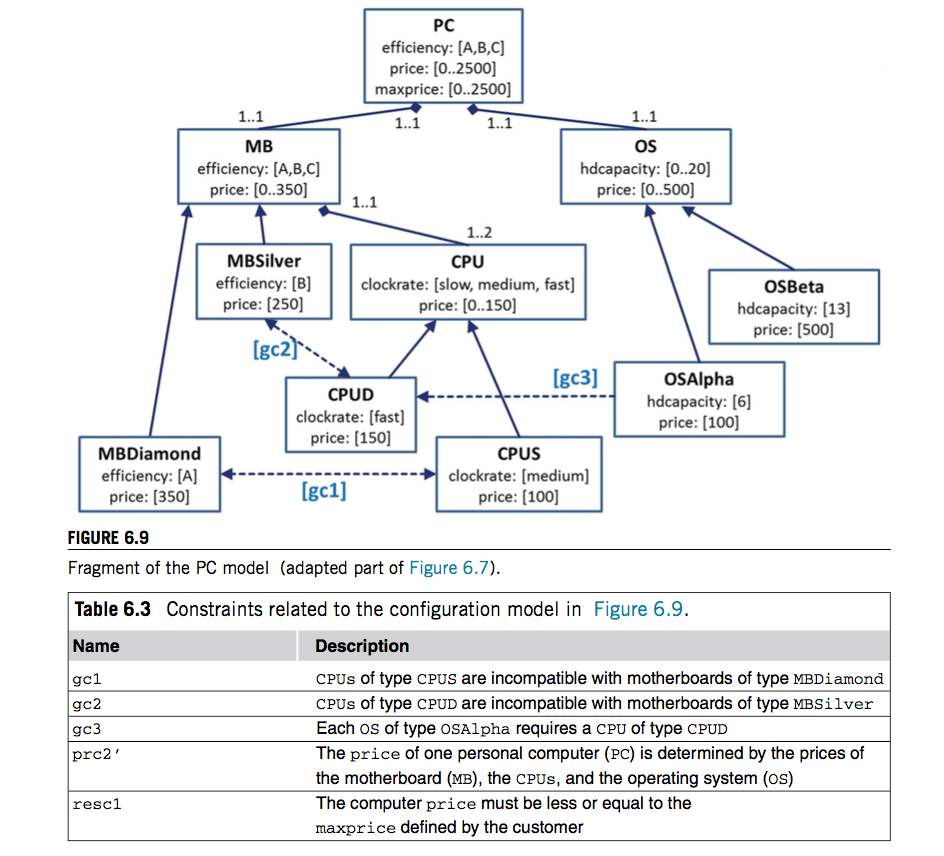
\includegraphics[width=0.9\linewidth]{Abbildungen/konfigurationsmodellUml.png}
	\captionof{figure}[konfigurationsmodellUml]{UML-Konfigurationsmodellvisualisierung einer PC-Konfiguration (Quelle: \cite{felferning14})}
	\label{fig:konfigurationsmodellUml}
\end{minipage}
\vspace{1em}

Abbildung \ref{fig:konfigurationsmodellUml} besteht aus einer Strukturdarstellung und einer Regeltabelle. Vor der genauen Beschreibung der Modellierungsmöglichkeiten erfolgt zur besseren Nachvollziehbarkeit eine unformale Beschreibung der Grafik:

Ein PC besteht aus einem Motherboard (MB) und Betriebssystem (OS). Ein Motherboard besitzt wiederum einen oder zwei CPUs. Ein Motherboard kann in der Ausfertigung "MBDiamond" oder "MBSilver" vorliegen. Ein CPU in den Ausfertigungen "CPUD" oder "CPUS", ein Betriebssystem als OSBETA oder OSALPHA. MBDiamond und CPUS dürfen nicht gleichzeitig gewählt werden. Gleiches gilt für MBSilver und CPUD. Wird OSAlpha gewählt, muss CPUD auch gewählt werden. Der Preis errechnet sich aus der Summer der Einzelkosten des verwendeten Motherboards, Betriebssystems und der CPUs. Er darf das Preislimit des Kunden nicht überschreiten.

Es stehen folgende Modellierungsmöglichkeiten des Strukturteils zur Verfügung:
\begin{compactitem}
\item \textbf{Komponententypen:} Kann mit Klassen aus der Objektorientierten Programmierung verglichen werden. Es besitzt einen eindeutigen Namen (z.B. MB) und wird durch eine Menge Attribute beschrieben (z.B. efficiency und price). Ein Attribute hat einen Datentyp, welcher eine Konstante, ein Wertebereich oder eine Enumeration (z.B. efficiency kann die Werte 'A', 'B' oder 'C' annehmen) sein kann.
\item \textbf{Assoziationen mit Kardinalität:} Aus UML sind die Associationstypen Aggregation und Komposition bekannt. Im Rahmen der Konfigurationsmodellbeschreibung geschieht eine Beschränkung auf die Komposition. Auf diese Art und Weise steht jede Komponente in einer \glqq Teil-Ganzes\grqq{} Beziehung zu genau einer anderen Komponente. Kardinalitäten beschreiben Assoziationen noch näher, indem sie sie durch Mengeninformationen ergänzen (ein Motherboard hat ein bis zwei CPUs, welche zu genau einem Motherboard gehören).
\item \textbf{Generalisierung}: Stellt die Verbindungen zwischen einem spezialisierten Subtyp (z.B. OSAlpha) zu einem einem generalisierten Supertyp (z.B. OS) her. Sie ist disjunkt und vollständig. Disjunkt bedeutet, dass ein Supertyp genau einem seiner Subtypen zugewiesen werden kann. Vollständig bedeutet, dass die Subtypen alle Instanzen darstellen, die ein Supertyp annehmen kann.
\end{compactitem}

Die Darstellung wird ergänzt durch Konfigurationsregeln. Sie gelten zwischen Komponententypen und/oder deren Attribute. Wenn möglich, werden sie direkt im Diagramm dargestellt werden. Anderenfalls werden sie in einer Tabelle aufgelistet. Man unterscheidet unterschiedliche Arten von Konfigurationsregeln \citeauthor{felferning14}:

\begin{compactitem}
\item \textbf{Grafische Konfigurationsregeln $GC$:} Können im Gegensatz zu anderen Regeln direkt im UML-Diagramm dargestellt werden. Ansonsten entsprechen sie einem der folgenden Typen.
\item \textbf{Preisbildungs-Konfigurationsregeln $PRC$:} Nehmen eine Sonderstellung ein, da sie keinen direkten Einfluss auf die Kombinierbarkeit haben. Stattdessen kann aus der Auswertung dieser Regel eine Preisinformation gewonnen werden. Bei tatsächlichen Konfigurationsanwendungen sind Preisregeln jedoch meistens nicht Teil des Konfigurationsmodells. Der Konfigurator hat dann einen eigenen Mechanismus zur Preisbildung.
\item \textbf{Ressourcen-Konfigurationsregeln $RESC$:} Beschränken die Produktion und den Verbrauch bestimmter Ressourcen.
\item \textbf{Abhängigkeits-Konfigurationsregeln $CRC$:} Beschreiben, unter welchen Voraussetzungen zusätzliche Komponenten Teil der Konfiguration sein müssen.
\item \textbf{Kompatibilitäts-Konfigurationsregeln $COMPC$:} Beschreiben die Kompatibilität  oder Inkompatibilität bestimmter Komponenten. In der Regeln finden sich in einer Regeltabelle entweder erstere oder zweitere Art, je nachdem, was den selteneren Fall darstellt.
\end{compactitem}

Die Menge aller Konfigurationsregeln wird auch als Wissensbasis $C_{KB}$ beschrieben. Es gilt:

 $C_{KB} = GC \cup PRC \cup RESC \cup CRC \cup COMPC$

\textbf{Konfigurationsaufgabe}\\
\citet{mittal89} definieren einen Konfigurationsaufgabe wie folgt:
\begin{quote}
(A) a fixed, pre-defined set of components, where a component is described by a set of properties, ports for connecting it to other components, constraints at each port that describe the components that can be connected at that port, and other structural constraints; (B) some description of the desired configuration; and (C) possibly some criteria for making optimal selections.
\end{quote}
(A) entspricht den Informationen, die aus dem oben vorgestellte Konfigurationsmodell resultieren. (B) und (C) sind als Kundenanforderungen zusammenfassbar. Informell wird daher die Aussage getroffen, dass eine Konfigurationsaufgabe aus den Konfigurationsmodell sowie den Kundenanforderungen besteht \citep{felferning14}.

Auf formeller Ebene ist eine Konfigurationsaufgabe auch auf Grundlage eines \ac{CSP} als \glqq Regelbasierte Wissensrepräsentation\grqq{} beschreibbar. Eine Diskussion dieser Variante ist sinnvoll, da so die Konfigurationslösung definiert werden kann. Es handelt sich dabei um ein Problem, bei dem für eine gegebene Menge Variablen und deren Wertebereiche unter Berücksichtigung einer Regelmenge versucht wird, eine zulässige Kombination von Werten aus den Wertebereichen der Variablen zu ermitteln. Bei einer Konfigurationsaufgabe wird die Regelmenge um die Menge der Kundenanforderungen erweitert \citep{felferning14}.

Eine Konfigurationsaufgabe ist demzufolge ein Tripel $(V, D, C)$, wobei $V = \{v_1, ..., v_n\}$ eine endliche Menge Variablen ,  $D  = \{dom(v_1), ..., dom(v_n)\}$ die Menge der Werte der Variablen und $C = C_{KB} \cup REQ$, wobei $C_{KB}$ die oben beschriebene Wissensbasis und $REQ$ die Menge der Kundenanforderungen ist \citep{felferning14}.

\textbf{Konfigurationslösung}\\
Auf Grundlage des \ac{CSP} kann eine Konfigurationslösung formell definiert werden. Es handelt sich dabei um eine Insttanziierung $I = \{v_1 = i_1, ..., v_n = i_n\}$, wobei $i_j$ ein Element aus $dom(v_1)$ ist. I ist vollständig (jede Variable bestitzt einen zugewiesenen Wert) und konsistent (erfüllt alle Konfigurationsregeln) \citep{falkner11}. Eine solche Lösung wird im folgenden als valide bezeichnet.

Eine Lösung kann durch ein UML-Instanz-Diagramm visualisiert werden, wie Abbildung \ref{fig:konfigurationsmodellUmlLoesung} darstellt. Anstatt von Komponententypen sind nur noch konkrete Instanzen enthalten.

\vspace{1em}
\begin{minipage}{\linewidth}
	\centering
	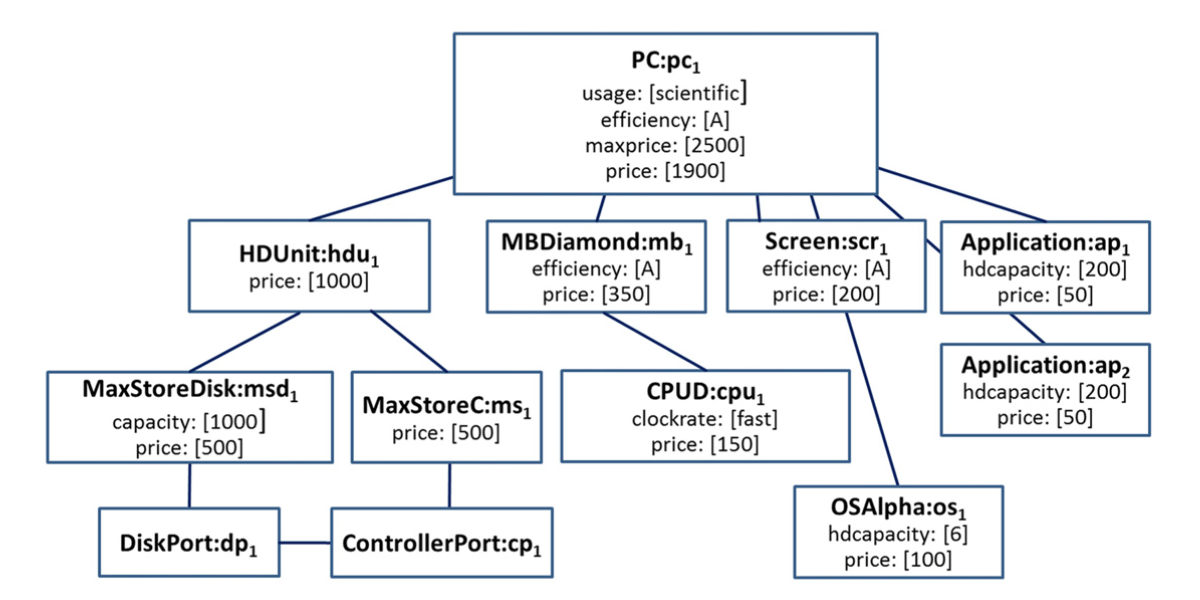
\includegraphics[width=0.9\linewidth]{Abbildungen/konfigurationsmodellUmlLoesung.png}
	\captionof{figure}[konfigurationsmodellUmlLoesung]{Visualisierung eines Konfigurationsergebnisses als UML-Instanz-Diagramm (Quelle: \cite{felferning14})}
	\label{fig:konfigurationsmodellUmlLoesung}
\end{minipage}
\vspace{1em}

Eine Konfigurationsaufgabe kann mehr als eine valide Lösung liefern. In diesem Falle ist es Möglich, dem Benutzer als Ergebnis eine Variantenmenge zu präsentieren. Nicht erfüllbare Constraints führen hingegen zu einer leeren Lösungsmenge.

Diese Beschreibung einer Konfigurationslösung suggeriert, dass zu Beginn des Konfigurationsprozesses einmalig die Kundenanforderungen aufgenommen und daraufhin die Lösungsmenge ermittelt wird. Diese Form ohne interaktive Eingriffsmöglichkeiten wird als statisch bezeichnet. Demgegenüber erlaubt die interaktive Konfiguration das schrittweise Treffen und Revidieren von Entscheidungen \citep{hadzic04}. Dieser Prozess muss durch eine Software unterstützt werden. Sie wird als Konfigurator bezeichnet und wird im Folgenden vorgestellt.

\subsubsection{Konfigurator}
Der Konfigurator ist das System, welche die Schnittstelle zum Benutzer darstellt und den Konfigurationsprozess durchführt. Es bekommt die Konfigurationsaufgabe als Eingabe und liefert als Ausgabe die Konfigurationslösung \citep{felferning14}. Sie "[...] führen den Abnehmer durch alle Abstimmungsprozesse, die zur Definition des individuellen Produktes nötig sind und prüfen sogleich die Konsistenz sowie Fertigungsfähigkeit der gewünschten Variante" \citep{piller06}.

Nach \citet{piller06} besitzt ein Konfigurator typischerweise drei Komponenten:
\begin{compactitem}
\item \textbf{Konfigurationskomponente:} Führt den Konfigurationsprozess durch. \citet{lutz11} bemerkt, dass hierzu eine explizite Wissensbasis (das Konfigurationsmodell, Anmerkung des Authors) und eine Problemlösungskomponente zur Lösungsfindung gehört.
\item \textbf{Präsentationskomponente:} Erstellte eine Konfiguration in Zielgruppenspezifischer Form. Der Author bemerkt, dass sie gleichzeitig als Schnittstelle zur Aufnahme der Kundenanforderungen dienst.
\item \textbf{Auswertungskomponente:} Präsentation der Konfiguration in einer Form, welche eine Interpretation der letztendlichen Variantenausprägung außerhalb des Konfigurators erlaubt. Dies können zum Beispiel Stücklisten, Konstruktionszeichnungen oder Arbeitspläne sein.
\end{compactitem}

Konfiguratoren für die Erhebung komplexer Anforderungen technischer Systeme unterschieden müssen von Konfiguration für den Einsatz im \ac{MC} werden \citep{felferning14}. Erstere sind für den Experteneinsatz gedacht oder dienen nach \citet{piller06} als Vertriebskonfiguratoren der Unterstützung des Verkaufsgespräches.   Letztere werden von Kunden in einer Company-to–Customer Beziehung genutzt und werden auch als Mass Customization Toolkit bezeichnet. Die sogenannte Selbstkonfiguration ist wesentlich sie die Verheiratung von kundenindividueller Fertigung und Massenproduktion, indem der zeitkonsumierende Prozess der Erhebung der Kundenbedürfnisse auch die Seite des Kunden verlagert wird\citep{piller06}

Konfiguratoren können bei allen in Abschnit \ref{subssubsection:Produktklassifizierung} genannten Produktionskonzepten zum Einsatz kommen. Je nach Produktionskonzept erfüllen sie für den Anwender eine unterschiedliche Funktion. Bei \ac{PTO} erfüllt der Konfigurator eine Katalogfunktion, indem er den Anwender er den Anwender bei der Auswahl eines fertigen Produktes aus einer Produktpalette unterstützt. Bei \ac{ATO} verhält sich der Konfigurator wie eine Variantengenerator, der den Anwender bei der Auswahl der richtigen, vom Hersteller vordefinierten Variante unterstützt. Der Anwendungsfall \ac{MTO} ist ähnlich, jedoch sind die Varianten vom Anwender definiert. Bei \ac{ETO} können Konfiguratoren durch den erheblichen Neukonstruktionsbedarf nur begrenzten Beitrag leisten. Aus dieser Erläuterung lässt sich Ableiten, dass das Haupteinsatzgebiet von Konfiguratoren im \ac{ATO}/\ac{MTO} Umfeld liegt.
\pagebreak

\subsection{Webservices}

Das \citet	{w3c04} definiert Webservices lose als:

\begin{quote}
\glqq [...] a software system designed to support interoperable machine-to-machine interaction over a network\grqq
\end{quote}

Die Definition schließt die Kommunikation heterogener Systeme ein. \glqq Zwischen Systemen\grqq{} differenziert gleichzeitig klar zur klassischen Verwendung eines Programms, bei der ein (menschlicher) Nutzer mit einem System kommuniziert. \citet{tilkov11} bemerkt, dass Web Service damit sehr weich definiert ist; \glqq nämlich eigentlich gar nicht\grqq{}. Fest steht, dass hier ein Service einen Dienst anbietet, der von einem Clienten über Webtechnologien angesprochen werden kann. Webservices sind demzufolge eine Möglichkeit zur Realisierung von Integrationsszenarien webbasierter Systeme.

\vspace{1em}
\begin{minipage}{\linewidth}
	\centering
	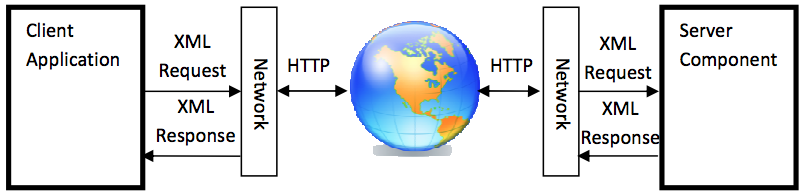
\includegraphics[width=0.7\linewidth]{Abbildungen/clientServerKommunikation.png}
	\captionof{figure}[clientServerKommunikation.png]{Generische Client-Server Kommunikation bei Webservices}
	\label{fig:clientServerKommunikation.png}
\end{minipage}
\vspace{1em}

Abbildung \ref{fig:clientServerKommunikation.png} entspricht im wesentlichen der klassischen Client-Server Kommunikation im Web. Exemplarisch werden XML-Daten übertragen, was die zugrunde liegende Idee der Webservices illustriert: die Übertragung anderer Daten als Webseiten mittels HTTP.

\citet{wilde11} reden von zwei etablierten \glqq Geschmäkern\grqq{} (flavors) in der Webservice Welt: SOAP und REST. Die erste Geschmacksrichtung bedeutet Web Services \glqq auf Basis von SOAP, WSDL und den WS-*Standards - bzw. [...] deren Architektur\grqq{} \citep{tilkov11}. Hier wird also ein XML-basierter Technologiestack beschrieben. REST hingegen ist ein Archikturstil, der 2000 in der Dissertation von \citeauthor{fielding00} vorgestellt wurde. Der Versuch, beide Varianten direkt gegenüberstellen stellen zu wollen, ist ein \glqq [...] klassischer Apfel-Birnenvergleich: ein konkretes XML-Format gegen einen abstrakten Architekturstil\grqq{} \citep{tilkov11}.

Vor einer detaillierteren Diskussion von SOAP und REST wird zur Einordnung eine grundlegende Unterscheidung der Ansätze vorgestellt. Gemeinsam ist beiden, dass HTTP als Transportprotkoll zur Übertragung der Frage (Request) verwendet wird, die vom Server (Response) beantwortert werden soll. HTTP wiederum besteht aus einem Header und einem Entity-Body zur Übertragung von Daten. \citet{richardson07} haben zwei Leitfragen herausgearbeitet, die von den jeweiligen Ansätzen unterschiedlich beantwortet werden: wo in diesem Paket sagt der Client dem Service, mit welchen Daten (Fokusinformation) was (Methodeninformation) gemacht werden soll?

Die Fokusinformation sagt aus, für welche Datenelemente sich der Client interessiert (z.B. ein Artikel eines Onlineshops). Bei REST ist dies der URI zu entnehmen (z.B. http://onlineshop.com/artikel/pc). Bei SOAP steht diese Information in einer XML-Datei welche Entity-Body übertragen wird; die sogenannte Payload. Die Methodeninformation sagt aus, was mit dem identifizierten Datenelement geschehen soll (Bsp:: lege einen neuen PC-Artikel an). Bei REST steht dies im Methodenfeld der HTTP-Headers, bei SOAP wieder im Entity-Body. Daraus lässt sich als grundlegender Unterschied ableiten: SOAP verwendet HTTP nur als Transportprotokoll, REST auch dessen Ausdruckskraft \citep{wilde11}.

\subsubsection{SOAP}
Bei SOAP-Web Services wird ein \ac{RPC} durchgeführt. Dabei handelt es sich um eine generelle Technik zur Realisierung von Systemverteilung. Ein System ruft die Funktion eines Systems aus einem anderen Adressraum auf. SOAP ist ein XML-basiertes Umschlagsformat, welches wiederum die Beschreibung eines Methodenaufrufs in XML-Form enthält. Bei SOAP-Web Services werden also \ac{RPC}s über HTTP getunnelt \citep{wilde11}. Das ist Konvention, aber keine Notwendigkeit: der SOAP-Umschlag ist Transportunabhängig, könnte also auch von anderen Protokollen als HTTP übertragen werden \citep{tilkov11}. Solange es sich bei dem Transportprotokoll um eine Webtechnologie handelt, wird die Webservicedefinition nicht verletzt.

Wie die Beschreibung des \ac{RPC} aussehen muss, definiert die \ac{WSDL}. Jeder SOAP basierte Service stellt eine machinenverarbeitbare \ac{WSDL}-Datei bereit. Darin werden die aufrufbaren Methoden, deren Argumente und Rückgabetypen beschrieben. Außerdem werden Schemata der XML-Dokumente festgehalten, die der Service akzeptiert und versendet \citep{richardson07}.

Es existieren eine Vielzahl von Middleware-Interoperabilitätsstandards, die mit dem \glqq WS-\grqq{} Prefix versehen sind. Diese sind \glqq XML-Aufkleber\grqq{} für den SOAP-Umschlag, die HTTP-Headern entsprechen \citep{richardson07}. Sie erweitern die Ausdrucksmöglichkeit des SOAP-Formats \citep{wilde11}. Beispielsweise erlaubt WS-Security die Berücksichtigung von Sicherheitsaspekten bei der Client-Server Kommunikation. Eine Übersicht der existierenden Standards ist dem Wiki für Webservices \citet{webServiceWiki09} zu entnehmen.

\subsubsection{REST}
\begin{quote}
\glqq Eine Architektur zu definieren bedeutet zu entscheiden, welche Eigenschaften das System haben soll, und eine Reihe von Einschränkungen vorzugeben, mit denen diese Eigenschaften erreicht werden können.\grqq{} \citep{tilkov11}
\end{quote}

Dies ist in der Dissertation von \citeauthor{fielding00} geschehen, in der REST als Architekturstil definiert wird. Ein Architekturstil ist ein stärkerer Abstraktionsgrad als eine Architektur. Beispielsweise ist das Web eine HTTP-Implementierung von REST \citep{tilkov11}. Tatsächlich wurden die Einschränkungen von REST aber dem Web entnommen, indem \citeauthor{fielding00} es post-hoc als lose gekoppeltes, dezentralisiertes Hypermediasystem konzeptualisiert \citep{wilde11} und dann von diesem Konzept abstrahiert hat. Einen Webservice nach dem REST-Architekturstil zu implementieren, bedeutet, es dem Wesen des Webs anzupassen und dessen stärken zu nutzen \citep{tilkov11}.

Entsprechend \citeauthor{tilkov11}s Architekturdefinition werden im Folgenden die Einschränkungen von REST sowie die daraus resultierenden Eigenschaften besprochen.

\textbf{Einschränkungen}\\
Einschränkungen sind - in eigenen Worten - Implementierungskriterien. Während \citeauthor{fielding00} in seiner theoretischen Abhandlung explizit vier solcher Kriterien nennt, basiert die folgende Auflistung auf der praxiserprobten Variante der Sekundärliteratur \citep{wilde11, tilkov11}.

\begin{compactitem}
\item \textbf{Ressourcen mit eindeutiger Identifikation}: \glqq Eine Ressource ist alles, was wichtig genug ist, um als eigenständiges Etwas referenziert zu werden\grqq{} \citep{richardson07}. Identifiziert werden sie im Web durch URIs, die einen globalen Namensraum darstellen.  Es ist hervorzuheben, dass Ressourcen nicht das gleiche sind wie die Datenelemente aus der Persistenzschicht einer Anwendung. Sie befinden sich auf einem anderen Abstraktionsniveau. Beispiel: eine Warenkorbressource kann eine Auflistung von Artikeln sein, welche allerdings nicht einzeln als Ressource ansprechbar sind. \citeauthor{tilkov11} nimmt in diesem Zusammenhang eine Typisierung von Ressourcen vor. Von den sieben verschiedene Ressourcentypen sind folgende im Rahmen der Fragestellung interessant:
\begin{enumerate}[a.]
\item Bei einer \textbf{Projektion} wird die Informationsmenge verringert, indem eine sinnvolle Untermenge der Attribute einer abgerufenen Ressource gebildet wird. Zweck ist die Reduktion der Datenmenge. Beispiel: Weglassen der Beschreibungstexte von Warenkorbartikeln.
\item Die \textbf{Aggregation} ist das Gegenteil. Hier werden Attribute unterschiedlicher Ressourcen zur Reduktion der Anzahl notwendiger Client/Server Interaktionen zusammengefasst. Beispiel: Hinzufügen der Versandkosten beim Abruf der Warenkorbartikel.
\item \textbf{Aktivitäten} sind Ressourcen, die sich aus Prozessen ergeben, wie etwa ein Schritt innerhalb einer Verarbeitung. Beispiel: Ein Schritt einer nicht abgeschlossenen Konfiguration.
\end{enumerate}
\item \textbf{Hypermedia} beschreibt das Prinzip verknüpfter Ressourcen. So wird dem Client ermöglicht, neue Ressourcen zu entdecken oder bestimmte Prozesse anzustoßen. Beispiel: Zur einer Bestellbestätigungsressource wird der zugehörige Stornierungslink hinzugefügt.
\item \textbf{Standardmethoden/uniforme Schnittstelle}: Oben wurde beschreiben, dass jede Ressource durch (mindestens) eine ID identifiziert wird. Jede URI unterstützt dabei den gleichen Methodensatz, welche mit den HTTP-Methoden korrespondieren. Das bedeutet - übertragen auf die objektorientierte Programmierung: jedes Objekt implementiert das gleiche Interface. Folgende Teilmenge der neun verfügbaren HTTP-Methoden finden in der Literatur am häufigsten Erwähnung:
\begin{enumerate}[a.]
\item \textbf{GET:} Das Abholen einer Ressource.
\item \textbf{PUT:} Das Anlegen oder Aktualisieren einer Ressource. Je nachdem, ob unter dieser URI bereits eine Ressource existiert.
\item \textbf{POST:} Bedeutet im engeren Sinne das Anlegen einer Ressource unter einer URI, die vom Service bestimmt. Im weiteren Sinne kann durch Post ein Prozess angestoßen werden.
\item \textbf{Delete:} Das Löschen einer Ressource.
\end{enumerate}

\vspace{1em}
\begin{minipage}{\linewidth}
	\centering
	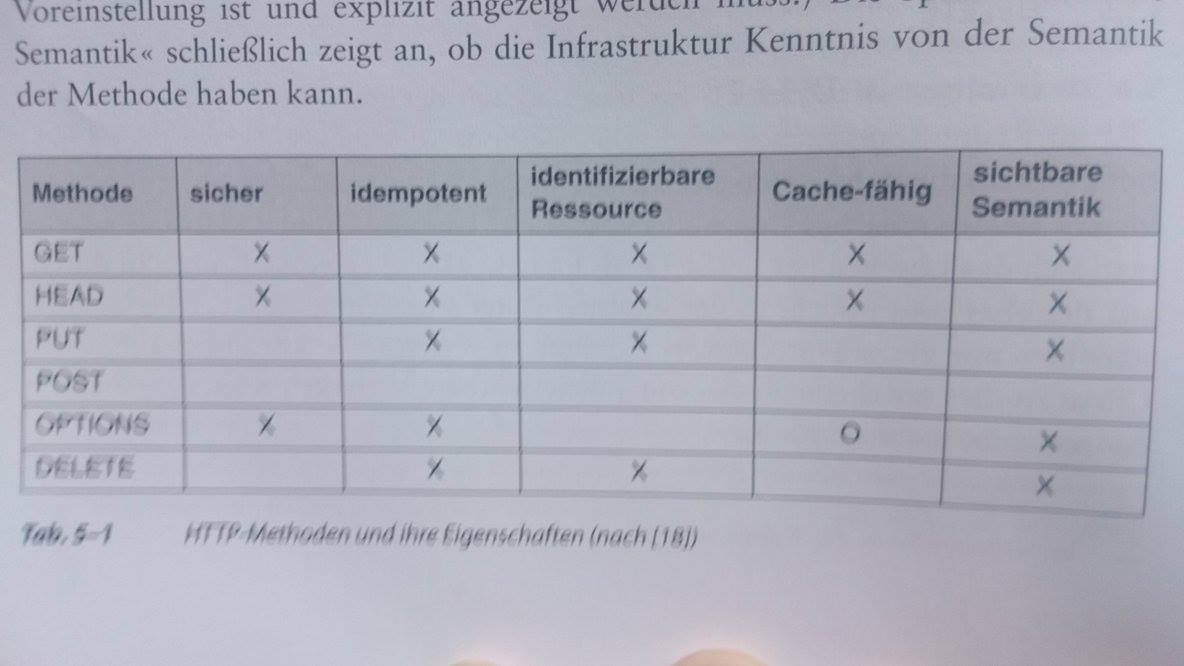
\includegraphics[width=0.7\linewidth]{Abbildungen/restMethoden.jpg}
	\captionof{figure}[restMethoden]{HTTP-Methoden und ihre Eigenschaften
	\footnote{Relevante Attribute im Rahmen der Fragestellung: \glqq sicher\grqq{} bedeutet Nebenwirkungsfrei, d.h. kein Ressourcenzustand ändert sich durch diese Methode. \glqq Idempotent\grqq{} bedeutet, dass das Resultat der Methode bei Mehrfachausführung das gleiche ist. \glqq Identifizierbare Ressource\grqq{} bedeutet, dass die URL garantiert eine Ressource identifiziert.}
	(Quelle: \citet{tilkov11})}
	\label{fig:restMethoden}
\end{minipage}
\vspace{1em}

Abbildung \ref{fig:restMethoden} fast die Eigenschaften der Methoden aus der HTTP-Spezifikation 1.1 zusammen. Die Implementierung einer Methode muss dem erwarteten Verhalten aus dieser Spezifikation entsprechen. Die Praxis zeigt, dass nur die Methoden unterstützt werden, die für die jeweilige Ressource sinnvoll sind. Abbildung \ref{fig:restMethoden} macht außerdem klar, dass es für POST keinerlei Garantien gibt. Da nicht eindeutig ist, ob über POST eine Ressource erstellt oder ein Prozess angestoßen wird, sehen \citeauthor{richardson07} hierin eine Verletzung der uniformen Schnittstelle. Dies bedeutet in der Praxis: was bei einem Post passiert, ist nicht der HTTP-Spezifikation, sondern der API-Beschreibung des Webservice zu entnehmen.
\item \textbf{Ressourcen und Repräsentationen:} Beschreibt die Darstellungen einer Ressource in einem definierten Format. Der Client bekommt nie die Ressource selbst, sondern nur eine Repräsentation derer zu sehen. In der Praxis wird meist eine  serialisierte Variante eines Objektes als JSON zur Verfügung gestellt. Beispiel: Bereitstellung einer Bestellbestätigung als PDF und HTML.
\item \textbf{Statuslose Kommunikation} bedeutet die Nichtexistenz eines serverseitig abgelegten, transienten, clientspezifischen Status über die Dauer eines Requests hinweg. Der Service benötigt also nie Kontextinformationen zur Bearbeitung eines Requests. Beispiel: Ein Warenkorb wird nicht in einem Sessionobjekt, sondern als persistentes Datenelement gehalten.
\end{compactitem}

Diese Auflistung legt folgende Frage nahe: ist ein Webservice nur dann REST-konform, wenn alle Kriterien erfüllt werden? Was ist mit einem Webservice, der allen Einschränkungen gerecht wird, jedoch Ressourcen nur als JSON ausliefert - ein in der Praxis häufig anzutreffender Fall. Und dennoch ein Verstoß gegen die Forderung nach unterschiedlichen Repräsentationen. Aus diesem Grund existiert das \glqq Richardson Maturity Model\grqq{}, welches die abgestufte Bewertung eines Webservices nach dessen REST-Konformität erlaubt. Es wird im Auswertungsteil vorgestellt und zur Evaluierung der Implementierung genutzt.

\textbf{Eigenschaften}\\
Aus den vorgestellten Kriterien resultieren folgende Eigenschaften \citep{tilkov11},  welche die Vorteile REST-basierter Webservices gegenüber der SOAP-Konkurrenz darstellen \citep{richardson07}:

\begin{compactitem}
\item \textbf{Lose Kopplung:} Beschreibt isolierte Systeme mit größtmöglicher Unabhängigkeit, die über Schnittstellen miteinander kommunizieren. Hierzu tragen die Standardmethoden bei.
\item \textbf{Interoperabilität:} Beschreibt die Möglichkeit der Kommunikation von Systemen unabhängig von deren technischen Implementierung. Dies ergibt sich durch die Festlegung auf Standards. Bei der Anwendung von REST auf Webservices sind dies die Webstandards (z.B. HTTP, URIs).
\item \textbf{Wiederverwendbarkeit}: Jeder Client, der die Schnittstelle eines REST-basierten Service verwenden kann, kann auch jeden anderen beliebigen REST-basierten Service nutzen - vorausgesetzt, das Datenformat wird von beiden Seiten verstanden.
\item \textbf{Performance und Skalierbarkeit}: Im Ideal sollen Webservices schnell antworten, unabhängig von der Anzahl von Anfragen in einem definierten Zeitraum. Dies wird durch Cachebarkeit (siehe HTTP-Methodenspezifikation) und Zustandslosigkeit erreicht. Da der Service keinen clientspezifischen Kontext aufbauen muss, müssen aufeinanderfolgende Requests nicht vom gleichen System beantwortet werden.
\end{compactitem}
\pagebreak

\subsection{Shopsysteme}

Im Folgenden wird durch die Charakterisierung des Begriffs eCommerce ein Andwendungsrahmen für eShops hergestellt. Deren softwaretechnische Umsetzung wird durch eShop-Systeme realisiert. Durch eine Kategorisierung der Systeme nach Anbieterstrategie wird abschließend die Menge der Open-Source-Lösungen für eine Konfiguratorintegration identifiziert.

\subsubsection{Anwendungsrahmen}
Eshops gehören zur Domäne des elektronischen Handels (eCommerce). Ecommerce ist \glqq die elektronisch unterstützte Abwicklung von Handelsgeschäften auf der Basis der Internet\grqq{} \citep{schwarze02}. Je nachdem, welche Marktpartner an dem Handelsgeschäft teilnehmen, werden verschiedene Formen des eCommerce unterschieden. Die in Abbildung \ref{fig:eCommerceGrundformen} fett hervorgehobenen Varianten werden von \citet{meier12} als \glqq die zwei Geschäftsoptionen des eCommerce\grqq{} bezeichnet: \ac{B2C} und \ac{B2B}. Bei \ac{B2C} erfolgt der Handel von Produkten und Dienstleistungen zwischen Unternehmen and Endverbraucher, bei \ac{B2B} zwischen Unternehmen.

\vspace{1em}
\begin{minipage}{\linewidth}
	\centering
	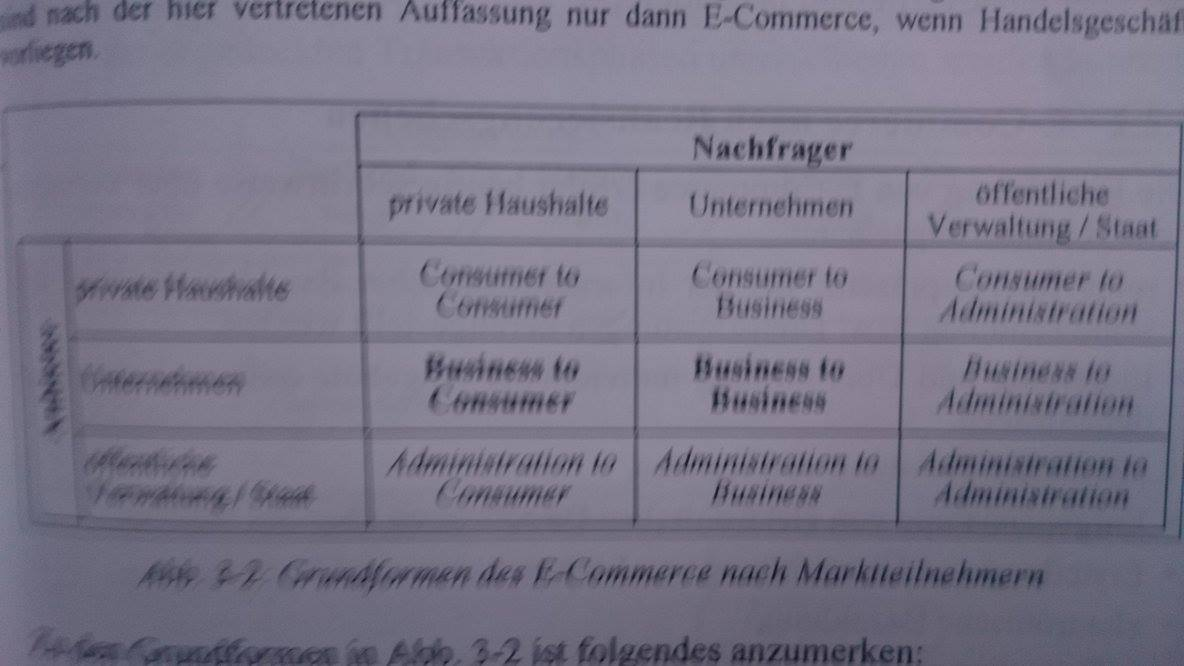
\includegraphics[width=0.7\linewidth]{Abbildungen/eCommerceGrundformen.jpg}
	\captionof{figure}[eCommerceGrundformen]{Grundformen des eCommerce nach Marktpartnern (Quelle: \citet{schwarze02})}
	\label{fig:eCommerceGrundformen}
\end{minipage}
\vspace{1em}

Für die Umsetzung von eCommerce existieren unterschiedliche Geschäftsmodelle. \citet{timmers98} nennt 11 verschiedene Formen. eShops sind eine eine davon. Es handelt sich dabei um ein \glqq Geschäftsmodell der Angebotsveröffentlichung, bei dem ein Anbieter seine Waren oder Dienstleistungen über das Web den Nachfragern offeriert\grqq{} \citep{bartelt00}.

Ein eShop bildet den traditionellen Einkaufsvorgang nach: Kunden können mittels einer Katalog- oder Suchfunktion über den Produktbestand navigieren. Produkte können ausgewählt und ausführliche, mit Medien angereicherte Beschreibungen abgerufen werden. Wunschartikel werden einem virtuellen Warenkorb hinzugefügt. Ist die Produktauswahl abgeschlossen, begibt sich der Kunde zur \glqq Kasse\grqq{}, wo die Zahlungsmodalitäten erledigt werden \citep{boles00}. Ein eShop beschreibt das Geschäftsmodell, jedoch noch nicht dessen Umsetzung als Softwaresystem. Diese wird als eShop-System bezeichnet \citep{boles00} und im Folgenden behandelt.

\subsubsection{eShop-Systeme}
\glqq eShop-Systeme sind Software-Systeme, die den Aufbau, die Verwaltung und den Einsatz von eShops unterstützen\grqq{} \citep{boles00}. Abbildung \ref{fig:eShopGrobarchitektur} zeigt die Grobarchitektur eines eShop-Systems nach \citeauthor{meier12}. Darin wird die Unterteilung zwischen Storefront und Backfront deutlich, welche in der Terminologie realer Shopsysteme als Front- und Backend bezeichnet werden \citep[vgl.][]{shopwareDoku}. Das Frontend ist der Interaktionsraum der Kunden, das Backend der adminsitrative Bereich des Shopbeitreibers.

\vspace{1em}
\begin{minipage}{\linewidth}
	\centering
	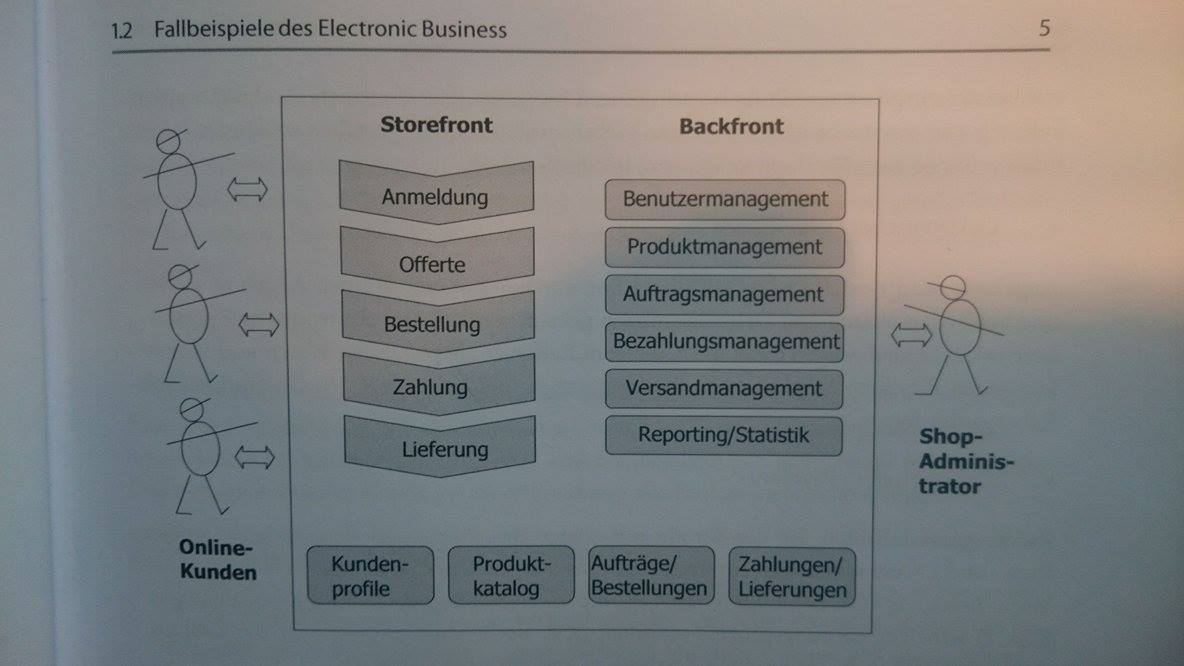
\includegraphics[width=0.7\linewidth]{Abbildungen/eShopGrobarchitektur.jpg}
	\captionof{figure}[eShopGrobarchitektur]{Grobarchitektur eines eShop-Systems (Quelle: \citet{meier12})}
	\label{fig:eShopGrobarchitektur}
\end{minipage}
\vspace{1em}

Die Hauptaufgaben eines eShop-Systems sehen \citet{boles00} in den Bereichen Merchandising (z.B. Management von hierarchisch strukturierten Produktkatalogen, Beeinflussung des Shopdesigns), Auftragsbearbeitung (z.B. Festlegung der Abarbeitungs-Pipeline, Integration von Bezahlverfahren) und Sonstiges (z.B. die Kopplung mit externen ERP-Systemen). Der konkrete Funktionsumfang hängt vom  gewählten eShop-System ab.

Die Systeme sind nach Strategie der Anbieter kategorisierbar:
\begin{compactitem}
\item \textbf{Open-Source}-Systeme sind kostenlos verfügbar. Sie bieten völlige Gestaltungsfreiheit, aber keinen Herstellersupport. Die Dokumentationen sind schwacher und der Funktionsumfang geringer als bei kostenpflichtigen alternativen. Andererseits existieren Communities, die Unterstützung bieten und die Entwicklung von Erweiterungen vorantreiben \citep{stahl15}. Beim kommerziellen Handel der modularen Erweiterungen auf shopspezifischen Stores liegt auch eine der wesentlichen Erlösquellen der Open-Source Strategie (z.B. der Addon Marketplace der \citeauthor{prestashopAddons} oder das Extensionverzeichnis der \citeauthor{opencartExtensions}).
\item \textbf{Kauf-Lösungen} können kostenpflichtig lizensiert werden (z.B. \citeauthor{shopwarePricing}). Sie bieten Herstellersupport, zusätzliche Dienstleistungen (z.B. Installation des Shops) und einen höheren Funktionsumfang (z. B. Schnittstellen zu verschiedenen Warenwirtschaftssystemen oder Zahlungsdienstleistern) \citep{stahl15}. Die Hersteller bieten verschiedene Editionen mit teilweise erheblichen Preisunterschieden an (Bsp.: die Preisdifferenz der Magento Enterprise Edition zu Enterprise Premium liegt bei über 35.000 \$, \citealp[vgl][]{fwpShop}).
\begin{enumerate}[a.]
\item Im Rahmen eines Dual-License-Modells ist eine Open-Source \textbf{Community Edition} Teil des Editionsspektrums \citep{t3n14} (vgl. das Shopangebot der \citeauthor{magentoShops}, \citeauthor{shopwarePricing} oder \citeauthor{oxidShops}). Durch den offenen Quellcode existiert auch hier der Handel modularer Erweiterungen, von dem auch die kostenpflichtigen Varianten profitieren (vgl. der Plugin Store der \citeauthor{shopwarePluginStore}). Aufgrund der gleichen Codebasis alles Editionen kann zu einer Kauf-Lösung migriert werden, was Flexibilität für  wachsende Shopanforderungen bietet.
\end{enumerate}
\item \textbf{Miet-Shops} entsprechen einer Cloud-Lösung als Software-as-a-Service (z.B. \citeauthor{stratoWebshops}, \citeauthor{shopify15}). Die technische Infrastruktur wird vom Provider zur Verfügung gestellt. Systemwartung, Bereitstellung der Shopsoftware und Hosting werden unter dem Mietpreis abgerechnet. \citet{stahl15} bewertet diese Variante als Einstiegslösung mit geringer Gestaltungsfreiheit.
\item \textbf{Eigenentwicklungen} eignen sich für individuelle Bedürfnisse, wenn die Standardsysteme die Anforderungen nicht mehr erfüllen \citep{stahl15, graf14}.
\end{compactitem}

Aus der Liste sind die (zumindest initial) kostenfreien Varianten ersichtlich: reine Open-Source eShop-Systeme sowie die Community-Editionen der Dual-License Modelle. Eine Anbieterübersicht ist \citet{t3n14} zu entnehmen. Eine Kategorisierung der Systeme nach Anforderungsklassen ist \citet{graf14} zu entnehmen.

\pagebreak
\section{Analyse}

\subsection{Tacton Produktkonfigurator}

\subsection{TCsite}

\subsection{Produktkonfiguration in TCsite}

\subsection{Shopsystem}

\pagebreak

\section{Anforderungen}

\subsection{Funktionale Anforderungen}

\subsection{Nichtfunktionale Anforderungen}

\pagebreak

\section{Integrationskonzept}

\pagebreak

\section{Integrationsumsetzung}

\pagebreak

\section{Fazit}

\pagebreak

% ----------------------------------------------------------------------------------------------------------
% Vorlagen
% ----------------------------------------------------------------------------------------------------------
\section{Vorlagen}
Dieses Kapitel enthält Beispiele zum Einfügen von Abbildungen, Tabellen, etc.

\subsection{Bilder}
Zum Einfügen eines Bildes, siehe Abbildung \ref{fig:osgi}, wird die \textit{minipage}-Umgebung genutzt, da die Bilder so gut positioniert werden können.

\vspace{1em}
\begin{minipage}{\linewidth}
	\centering
	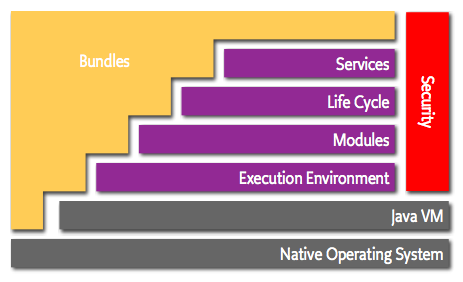
\includegraphics[width=0.7\linewidth]{Bilder/layering-osgi.png}
	\captionof{figure}[OSGi Architektur]{OSGi Architektur\footnotemark }
	\label{fig:osgi}
\end{minipage}
\footnotetext{Quelle: \url{http://www.osgi.org/Technology/WhatIsOSGi}}

\subsection{Tabellen}
In diesem Abschnitt wird eine Tabelle (siehe Tabelle \ref{tab:beispiel}) dargestellt.

\vspace{1em}
\begin{table}[!h]
	\centering
	\begin{tabular}{|l|l|l|}
		\hline
		\textbf{Name} & \textbf{Name} & \textbf{Name}\\
		\hline
		1 & 2 & 3\\
		\hline
		4 & 5 & 6\\
		\hline
		7 & 8 & 9\\
		\hline
	\end{tabular}
	\caption{Beispieltabelle}
	\label{tab:beispiel}
\end{table}

\pagebreak
\subsection{Auflistung}
Für Auflistungen wird die \textit{compactitem}-Umgebung genutzt, wodurch der Zeilenabstand zwischen den Punkten verringert wird.

\begin{compactitem}
	\item Nur
	\item ein
	\item Beispiel.
\end{compactitem}

\subsection{Listings}
Zuletzt ein Beispiel für ein Listing, in dem Quellcode eingebunden werden kann, siehe Listing \ref{lst:arduino}.

\vspace{1em}
\begin{lstlisting}[caption=Arduino Beispielprogramm, label=lst:arduino]
int ledPin = 13;
void setup() {
    pinMode(ledPin, OUTPUT);
}
void loop() {
    digitalWrite(ledPin, HIGH);
    delay(500);
    digitalWrite(ledPin, LOW);
    delay(500);
}
\end{lstlisting}

\subsection{Tipps}
Die Quellen befinden sich in der Datei \textit{bibo.bib}. Ein Buch- und eine Online-Quelle sind beispielhaft eingefügt.

Abkürzungen lassen sich natürlich auch nutzen. Weiter oben im Latex-Code findet sich das Verzeichnis.
\pagebreak

% ----------------------------------------------------------------------------------------------------------
% Literatur
% ----------------------------------------------------------------------------------------------------------
\renewcommand\refname{Quellenverzeichnis}
\bibliographystyle{myalpha}
\bibliography{bibo}
\pagebreak

% ----------------------------------------------------------------------------------------------------------
% Anhang
% ----------------------------------------------------------------------------------------------------------

\renewcommand\refname{Anhang}
\begin{appendix}
\chapter{Anhang}

\vspace{1em}
\begin{minipage}{\linewidth}
	\centering
	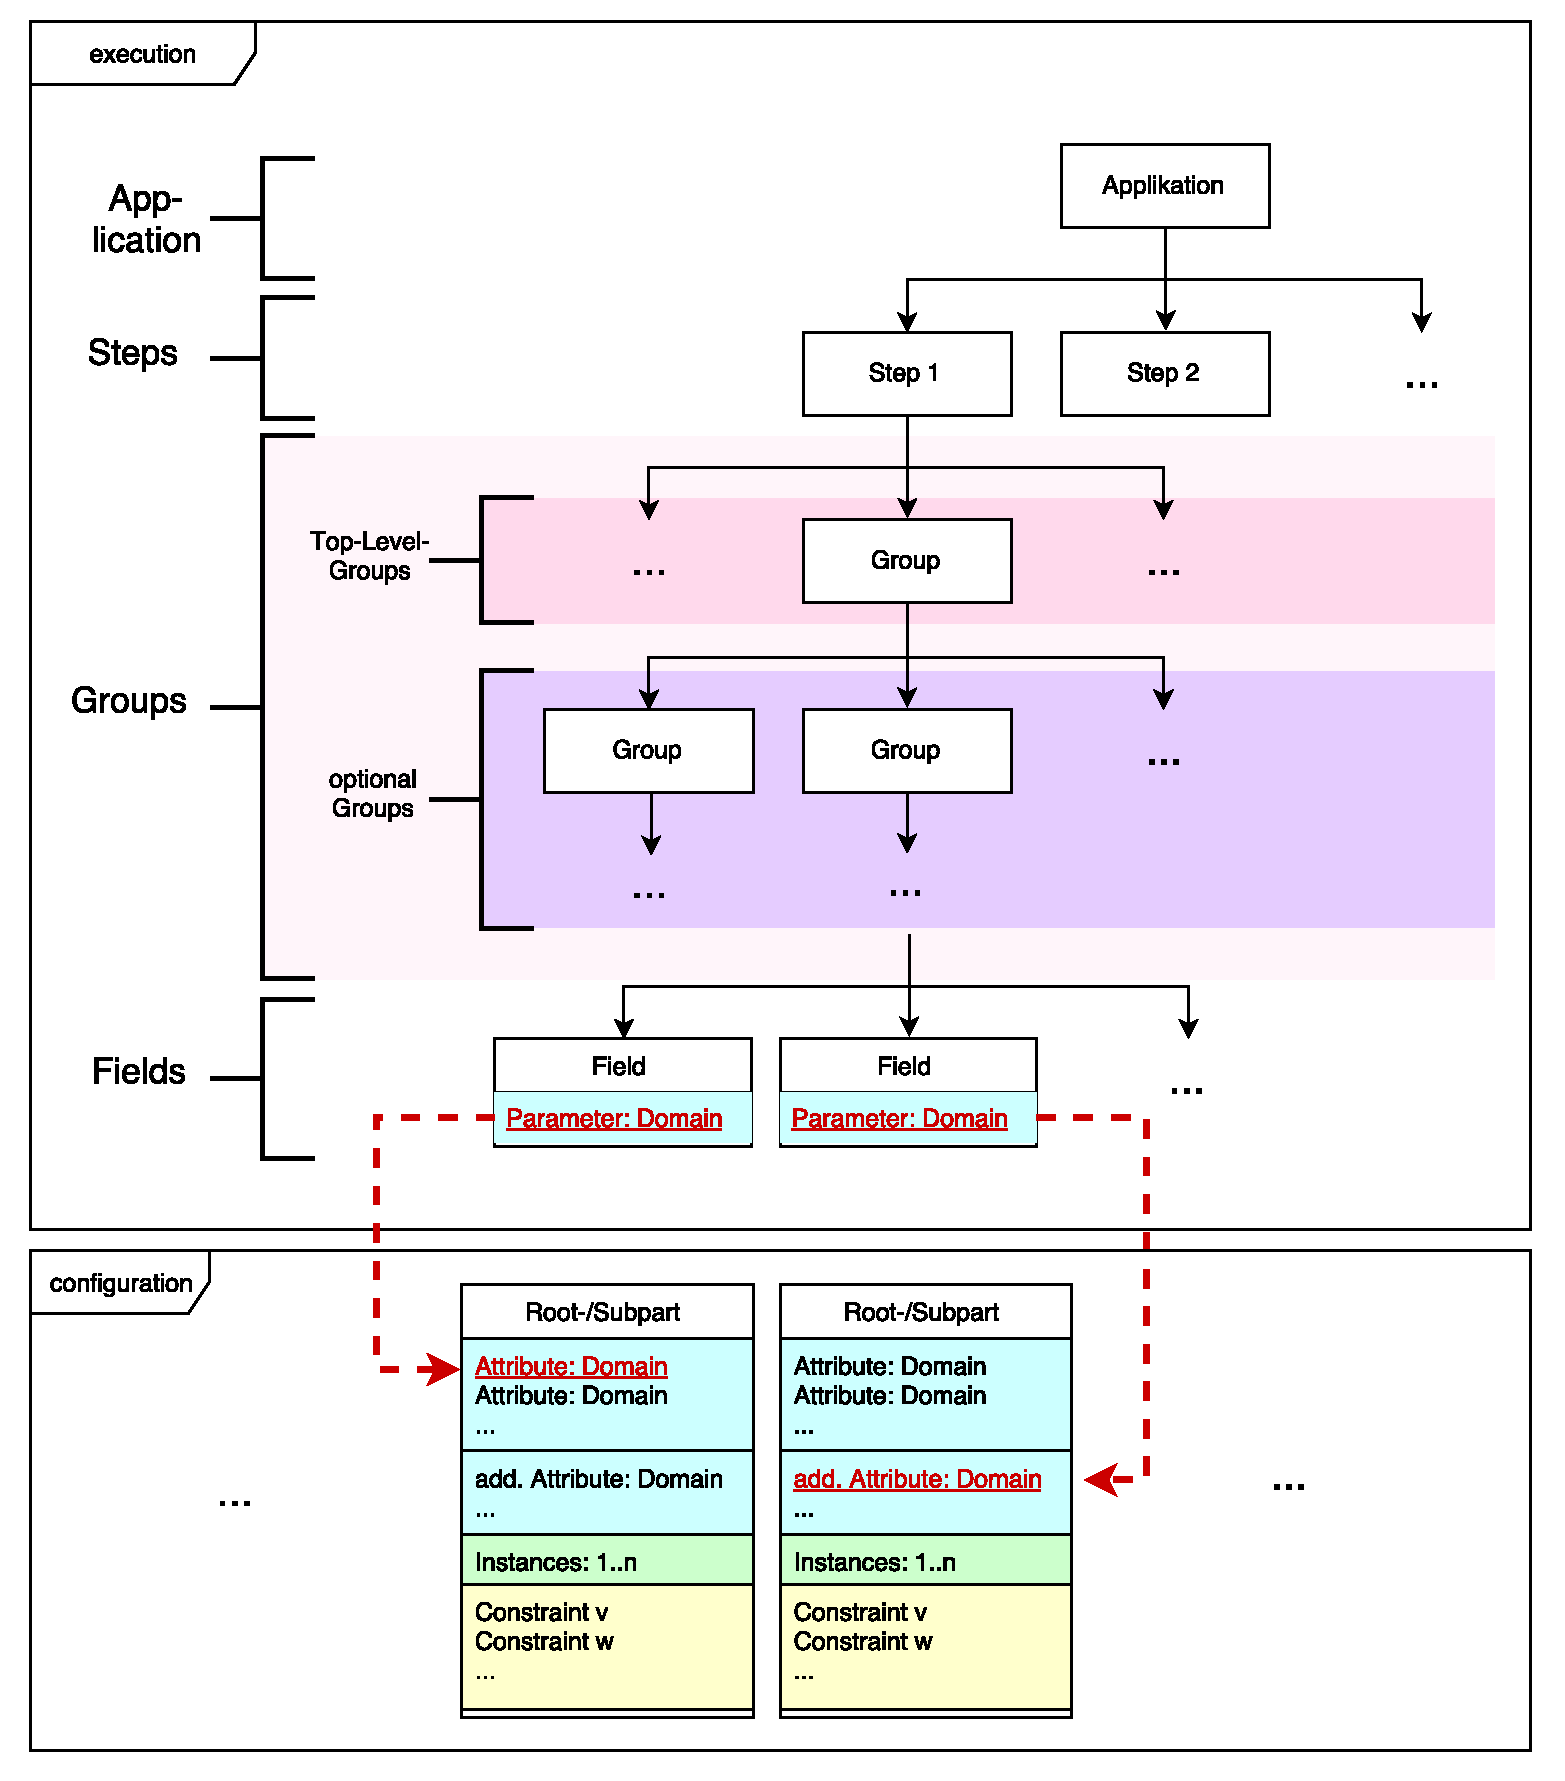
\includegraphics[width=1\linewidth]{Abbildungen/tactonModellExecution.pdf}
	\captionof{figure}[Vollständige Darstellung der generischen Execution-Struktur]{Vollständige Darstellung der generischen Execution-Struktur}
	\label{app:tactonModellExecutionLong}
\end{minipage}
\vspace{1em}

\vspace{1em}
\begin{minipage}{\linewidth}
	\centering
	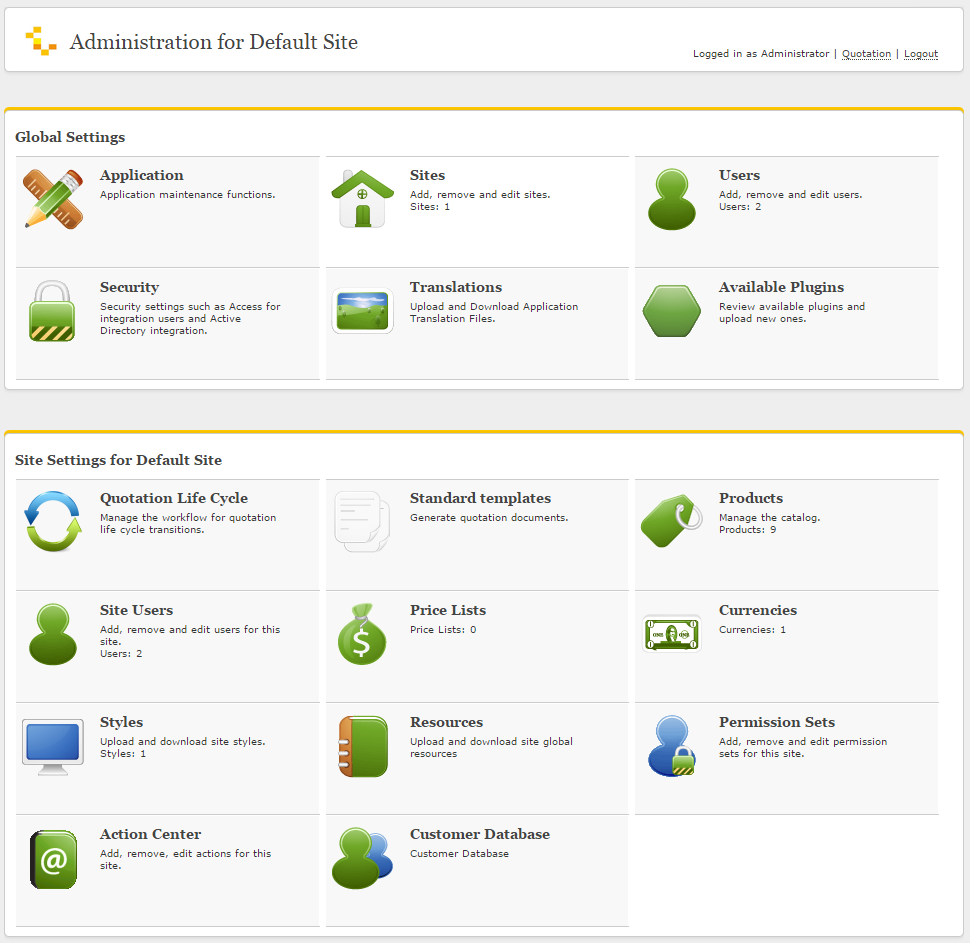
\includegraphics[width=1\linewidth]{Abbildungen/tcsiteAdministration.PNG}
	\captionof{figure}[tcsiteAdministration]{TCsite Administrationsoberfläche}
	\label{app:tcsiteAdministration}
\end{minipage}
\vspace{1em}

\vspace{1em}
\begin{minipage}{\linewidth}
	\centering
	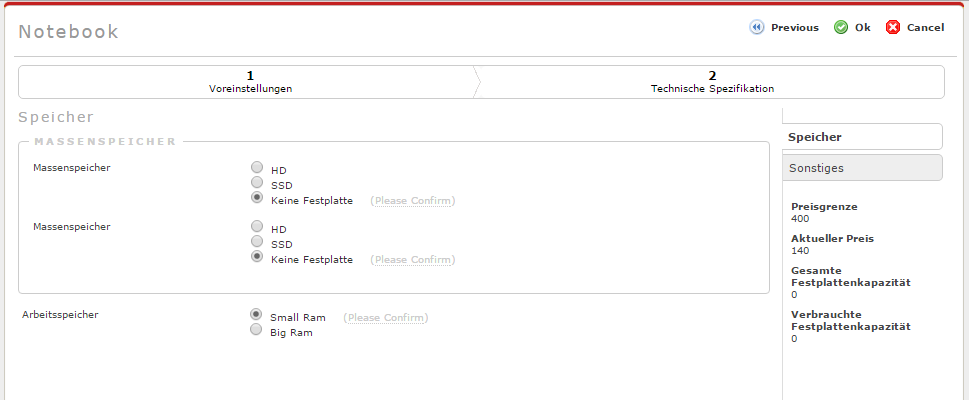
\includegraphics[width=1\linewidth]{Abbildungen/tcSiteConfigurationOptionalGroups.PNG}
	\captionof{figure}[tcSiteConfigurationOptionalGroups]{Darstellung optionaler Groups in TCsite}
	\label{app:tcSiteConfigurationOptionalGroups}
\end{minipage}
\vspace{1em}

\vspace{1em}
\begin{minipage}{\linewidth}
	\centering
	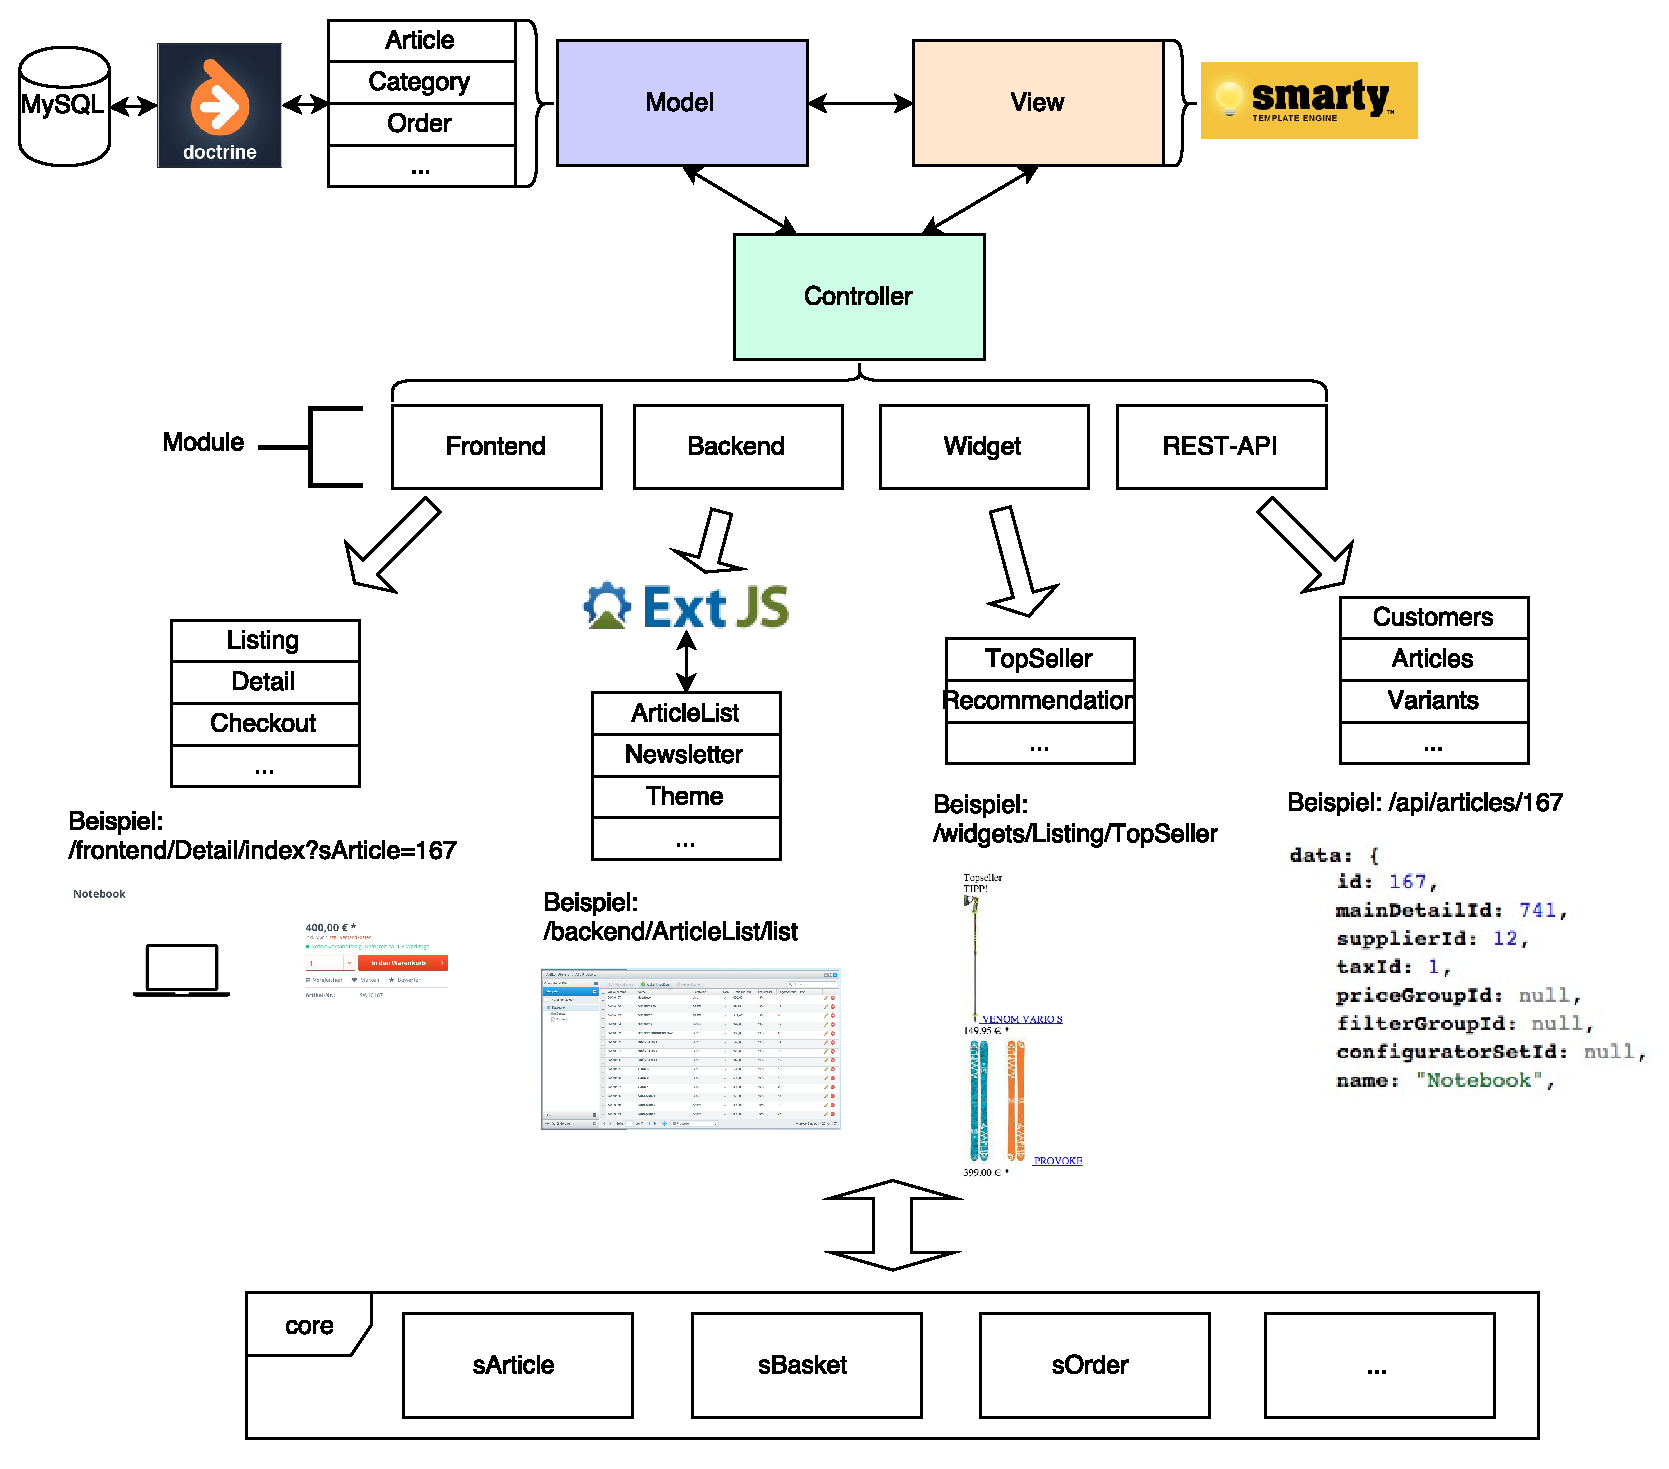
\includegraphics[width=1\linewidth]{Abbildungen/shopwareMVC.pdf}
	\captionof{figure}[vollständige High-Level-Architektur von Shopware]{vollständige Shopware High-Level-Architektur}
	\label{fig:shopwareMVCLong}
\end{minipage}
\vspace{1em}

\vspace{1em}
\begin{minipage}{\linewidth}
	\centering
	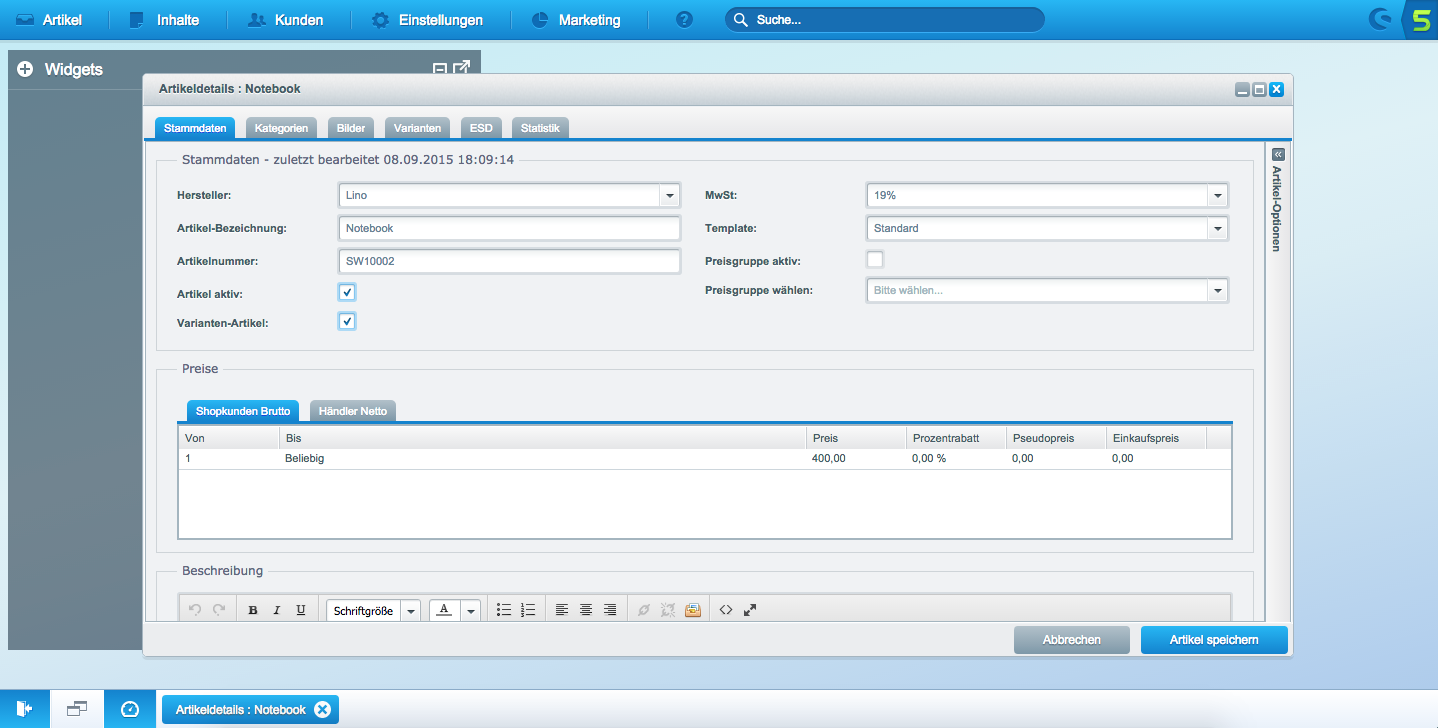
\includegraphics[width=1\linewidth]{Abbildungen/shopwareBackendArtikel.png}
	\captionof{figure}[shopwareBackendArtikel]{Anlegen eines Artikels im Backend}
	\label{app:shopwareBackendArtikel}
\end{minipage}
\vspace{1em}

\vspace{1em}
\begin{minipage}{\linewidth}
	\centering
	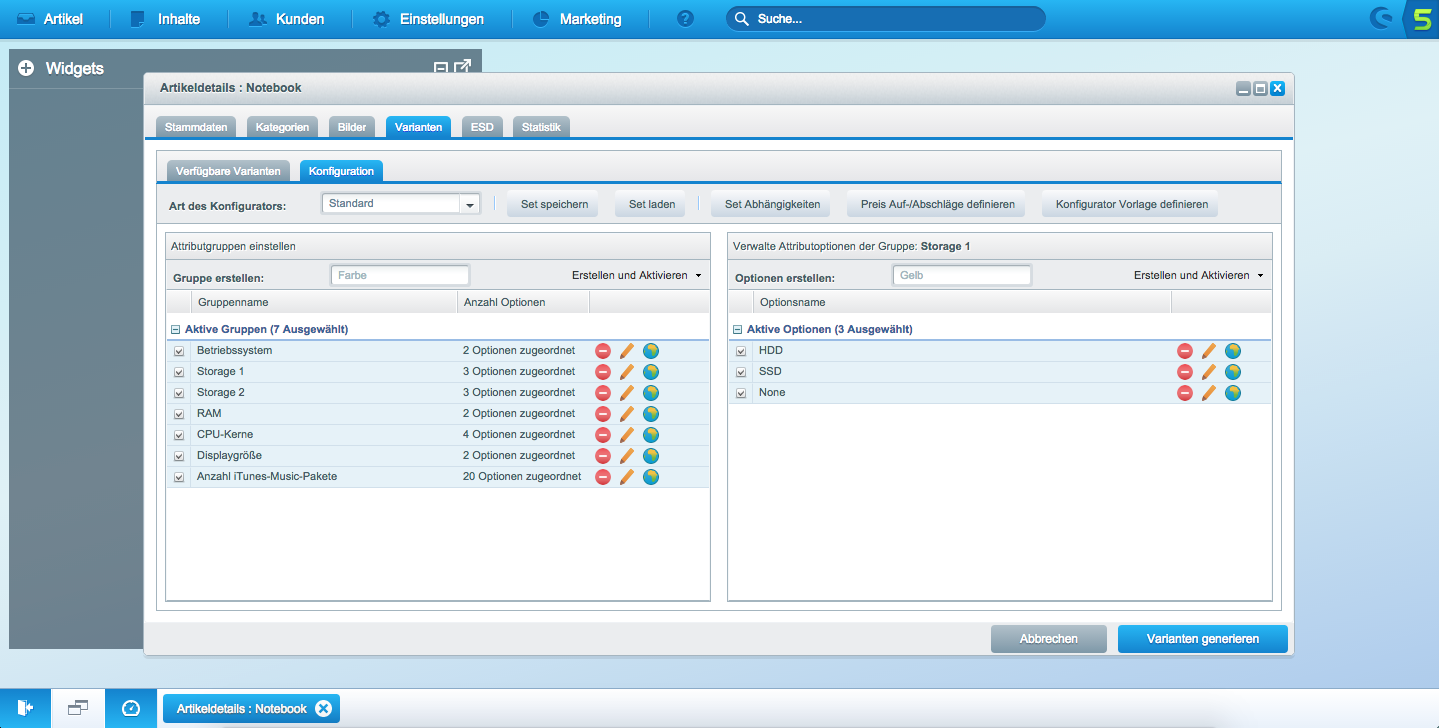
\includegraphics[width=1\linewidth]{Abbildungen/shopwareBackendArtikelVarianten.png}
	\captionof{figure}[shopwareBackendArtikelVarianten]{Generieren der Varianten im Backend}
	\label{app:shopwareBackendArtikelVarianten}
\end{minipage}
\vspace{1em}

\vspace{1em}
\begin{minipage}{\linewidth}
	\centering
	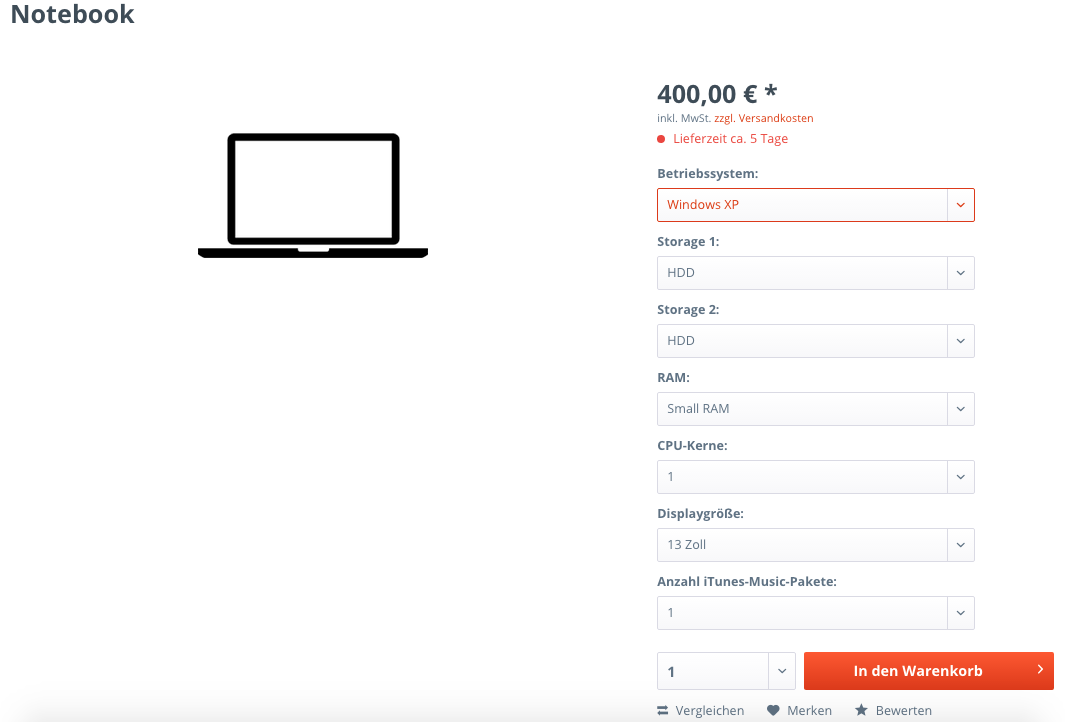
\includegraphics[width=1\linewidth]{Abbildungen/shopwareNotebookDetail.png}
	\captionof{figure}[shopwareNotebookDetail]{Detailansicht eines konfigurierbaren Notebooks in shopware.}
	\label{app:shopwareNotebookDetail}
\end{minipage}
\vspace{1em}

\vspace{1em}
\begin{minipage}{\linewidth}
	\centering
	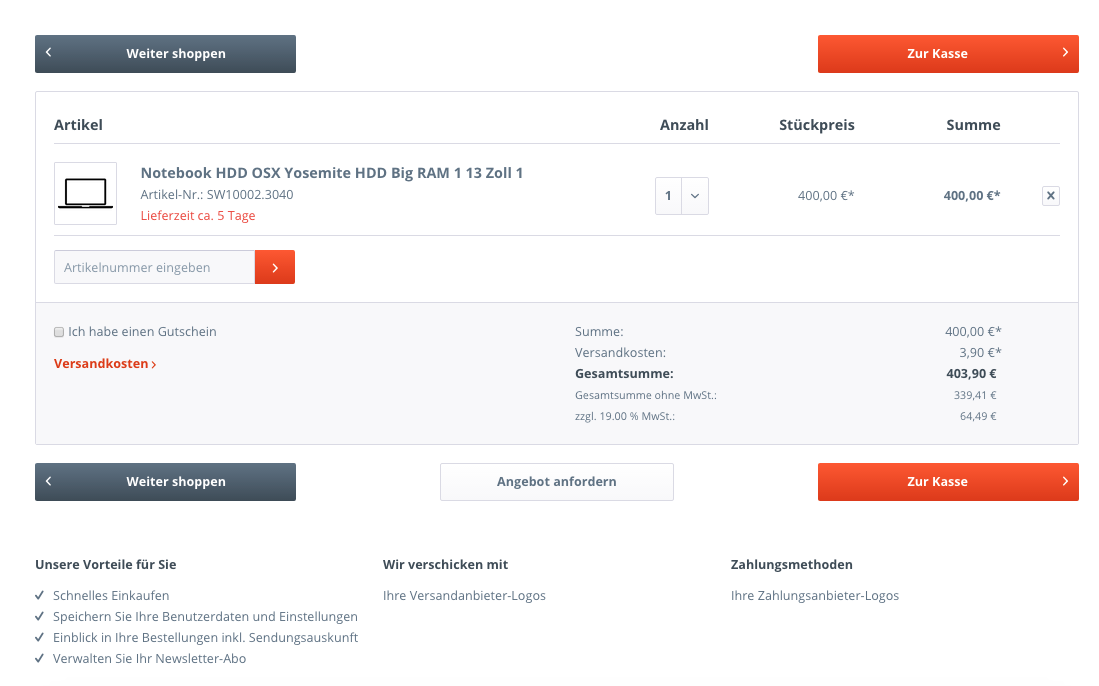
\includegraphics[width=1\linewidth]{Abbildungen/shopwareNotebookWarenkorb.png}
	\captionof{figure}[shopwareNotebookWarenkorb]{Warenkorb mit konfiguriertem Artikel.}
	\label{app:shopwareNotebookWarenkorb}
\end{minipage}
\vspace{1em}

\vspace{1em}
\begin{minipage}{\linewidth}
	\centering
	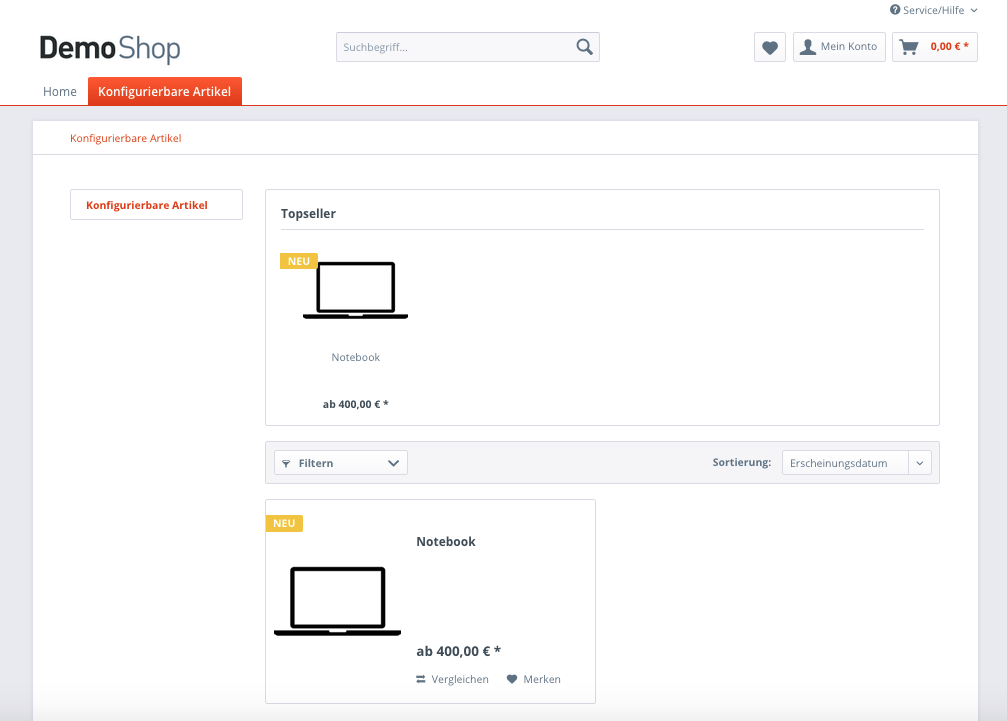
\includegraphics[width=1\linewidth]{Abbildungen/shopwareArtikelListing.png}
	\captionof{figure}[Artikellisting in Shopware]{Artikellisting in Shopware}
	\label{app:shopwareArtikelListing}
\end{minipage}
\vspace{1em}

\vspace{1em}
\begin{minipage}{\linewidth}
	\centering
	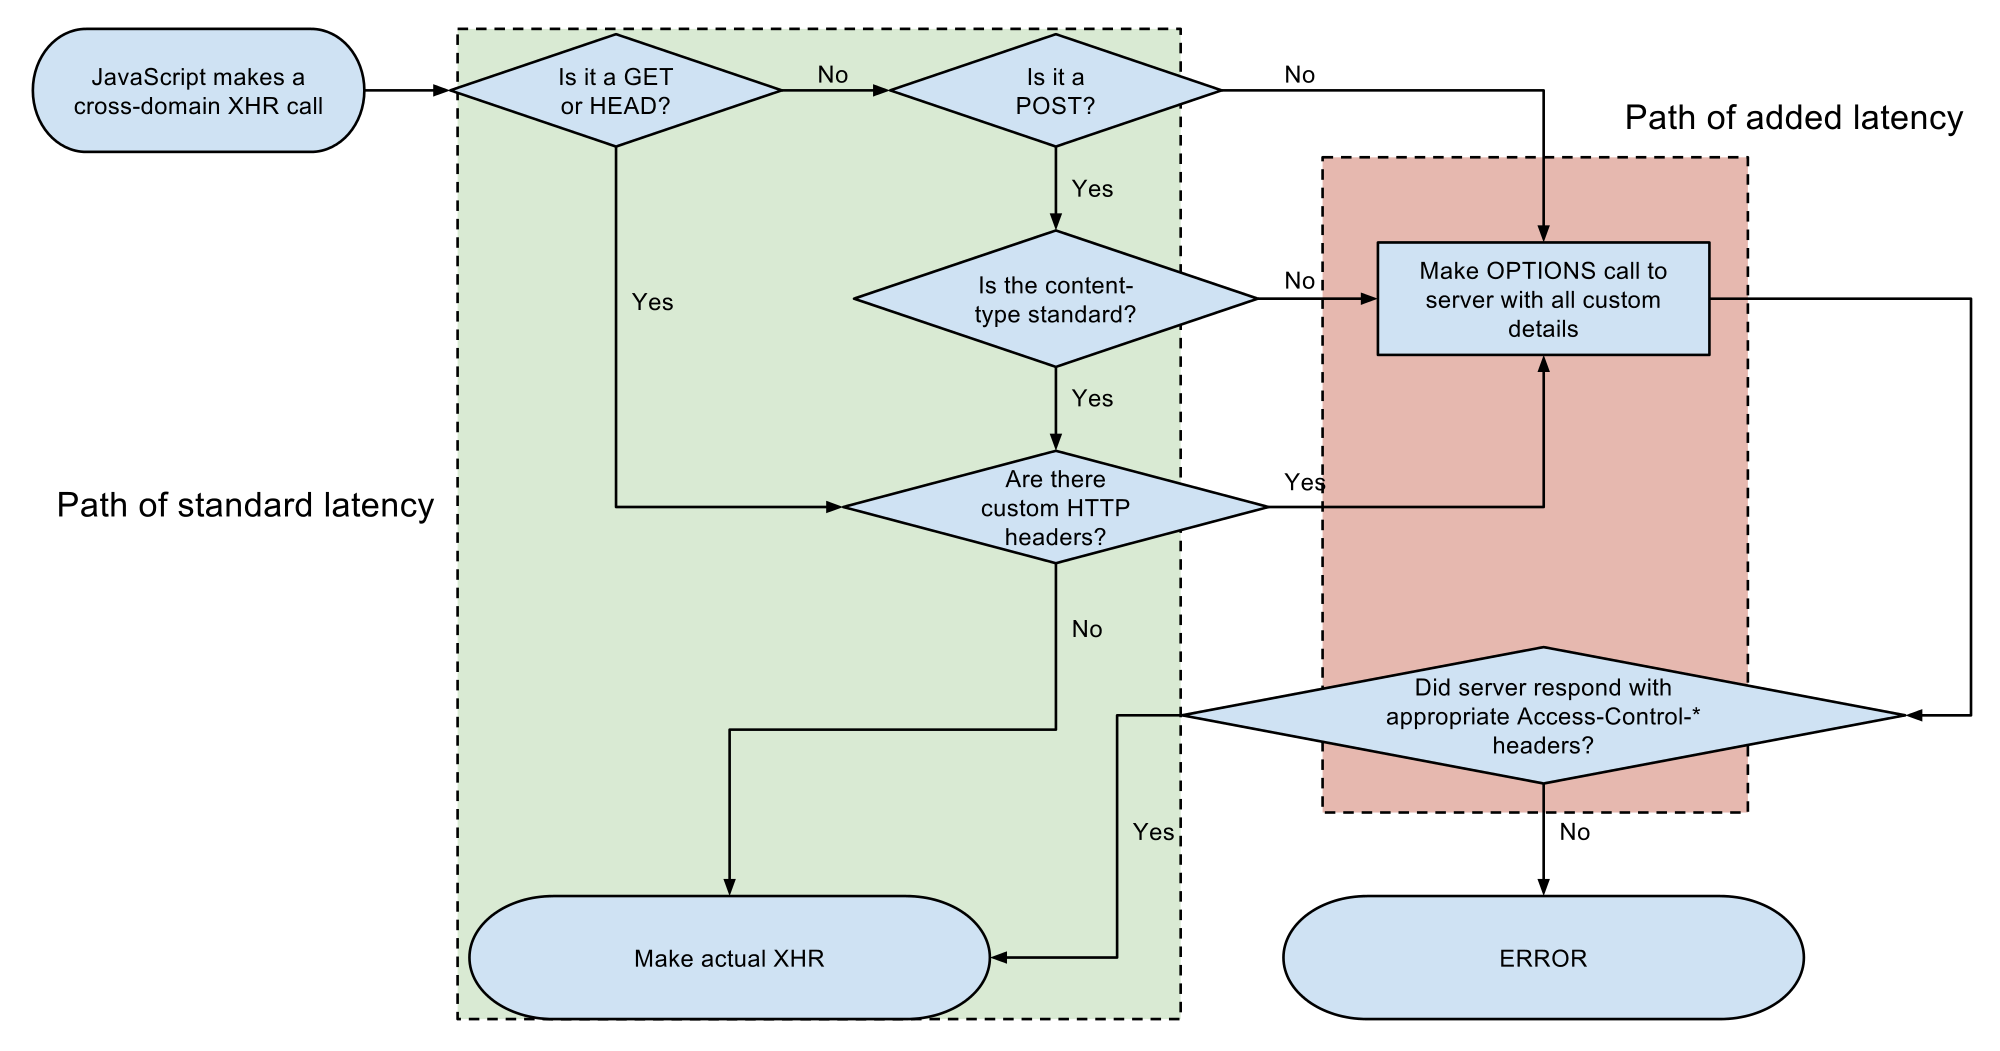
\includegraphics[width=1\linewidth]{Abbildungen/mozillaCORS.png}
	\captionof{figure}[mozillaCORS]{CORS-Flowchart.}
	\label{app:mozillaCORS}
\end{minipage}
\vspace{1em}

\end{appendix}

\chapter*{Selbstständigkeitserklärung}
\vspace{2em}
Ich versichere hiermit an Eides statt, dass ich die vorliegende Bachelorarbeit selbstständig und ohne unzulässige fremde Hilfe erbracht habe. Ich habe keine anderen als die angegebenen Quellen und Hilfsmittel benutzt sowie wörtliche und sinngemäße Zitate kenntlich gemacht. Die Arbeit hat in gleicher oder ähnlicher Form noch keiner Prüfungsbehörde
vorgelegen.

\vspace{4em}
\begin{minipage}{\linewidth}
	\begin{tabular}{p{15em}p{15em}}
		Datum: &  .......................................................\\
		& \centering (Unterschrift)\\
	\end{tabular}
\end{minipage}

\end{document}
